\pagecolor{CadetBlue!70!green}
\chapter{Bausteine von Algorithmen}
\label{kap:bausteinealgorithmen}

Mit dem Arduino und einigen einfachen Bauteilen lassen sich bereits zahlreiche Projekte umsetzen. Allerdings wird die Programmierung schnell unübersichtlich oder unnötig aufwendig, wenn man sich nicht mit algorithmischen Strukturen auskennt. Daher geht es im folgenden Kapitel um die Einführung von grundlegenden algorithmischen Bausteinen.

\bigskip
In diesem Kapitel lernst du\dots
\begin{itemize}
	\item \dots Entscheidungen zu programmieren,
	\item \dots den Arduino mit dem Computer kommunizieren zu lassen,
	\item \dots zwischen unterschiedlichen Datentypen zu unterscheiden,
	\item \dots Entscheidungen anhand mehrerer Kriterien zu treffen,
	\item \dots wie man Programme zur Planung oder zum Vergleich auf Papier einfach darstellen kann
	\item \dots Variablen zu benutzen,
	\item \dots zufällige Ereignisse zu programmieren,
	\item \dots mit Schleifen effizient zu programmieren,
	\item \dots systematisch nach Fehlern im Programm zu suchen.
\end{itemize}

\bigskip

\bigskip

\begin{projektueberblick}
	\item Fußgängerampel \dotfill \pageref{proj:fussampel}
	\item Juke-Box \dotfill \pageref{proj:jukebox}
	\item Straßenlampe \dotfill \pageref{proj:strassenlampe}
	\item Carport-Lampe \dotfill \pageref{proj:carportlampe}
	\item Auto-Blinker \dotfill \pageref{proj:blinker}
	\item Bombe bauen \dotfill \pageref{proj:bombe}
	\item Reaktionszeitmesser \dotfill \pageref{proj:reaktionszeitmesser}
	\item Reaktionsspiel \dotfill \pageref{proj:reaktionsspiel}
	\item Alarmanlage mit Lichtschranke \dotfill \pageref{proj:alarmanlage}
\end{projektueberblick}

\newpage
\nopagecolor
\section{Entscheidungen programmieren}
\label{sec:entscheidungen}

Schaltungen und Programme werden erst dann richtig interessant, wenn sie auf ihre Umwelt reagieren. Im einfachsten Fall lässt sich dazu ein Taster einbauen, mit dem von außen sich entscheiden lässt, wie das Programm weiterlaufen soll. Dementsprechend müssen im Programm \emph{Fallunterscheidungen} eingebaut werden.

\begin{ziel}
	\textbf{Ziel:} Der Arduino soll auf Eingaben aus seiner Umwelt reagieren.
\end{ziel}

\bigskip
\begin{projekt}[Fußgängerampel]\label{proj:fussampel}
	\begin{wrapfigure}{r}{0.4\textwidth}
		\centering
		\vspace{-2\baselineskip}
		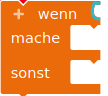
\includegraphics[width=0.15\textwidth]{./pics/wenn-mache-sonst.png}
		\label{abb:falls-dann}
	\end{wrapfigure}
	Baue und programmiere eine Fußgängerampel! Nutze dazu die Informationen aus dem Info-Kasten zum Taster.
\end{projekt}

\bigskip
\begin{zsfg}{Taster}
	\begin{minipage}{0.7\textwidth}
		Ein Taster ist wie ein Schalter, kann also geschlossen sein (Strom fließt) oder offen sein (Strom fließt nicht). Im Gegensatz zum Schalter springt ein Taster aber automatisch wieder in den offenen Zustand zurück, wenn er losgelassen wird.
	\end{minipage}
	\hfill
	\begin{minipage}{0.28\textwidth}
		\begin{minipage}{0.63\textwidth}
			\centering
			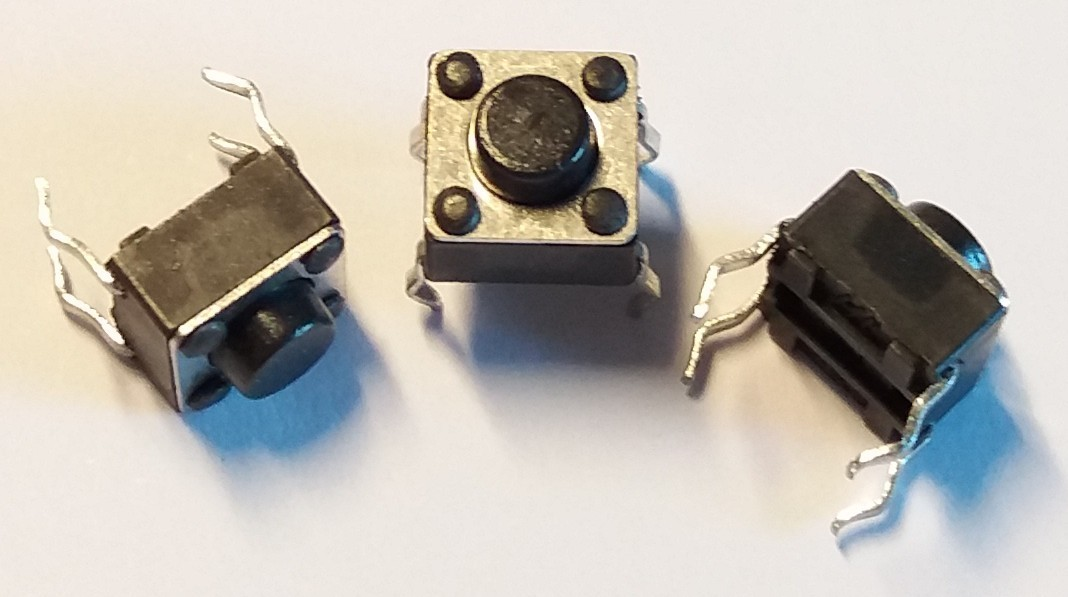
\includegraphics[width=\textwidth]{./pics/taster.jpg}
		\end{minipage}
		\hfill
		\begin{minipage}{0.33\textwidth}
			\centering
			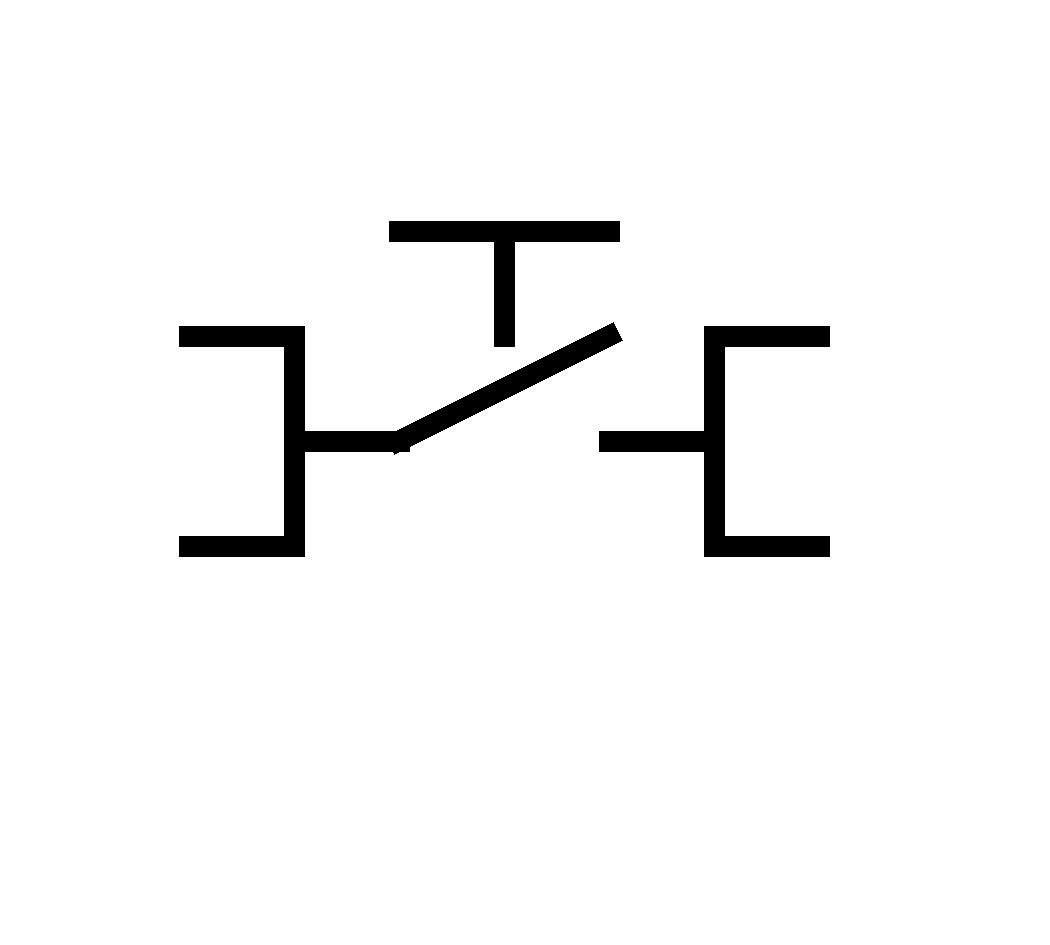
\includegraphics[width=\textwidth]{./Zeichnungen/taster-schaltsymbol.png}
		\end{minipage}
	\end{minipage}		
\end{zsfg}


\begin{minipage}{0.45\textwidth}
	In dem rechts abgebildeten Schaltplan ist dargestellt, wie man einen Taster am Arduino so anschließt, dass man seinen Zustand im digitalen Pin 3 auslesen kann. Unten ist die zugehörige Taster-Konfiguration abgebildet.
	
	\begin{figure}[H]
		\centering
		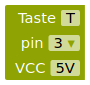
\includegraphics[width=0.3\textwidth]{./pics/tasterkonfiguration.png}
		\label{abb:tasterkonfiguration}
	\end{figure}

	\bigbreak
	\bigbreak
	\bigbreak
\end{minipage}
\hfill
\begin{minipage}{0.45\textwidth}
	\begin{figure}[H]
		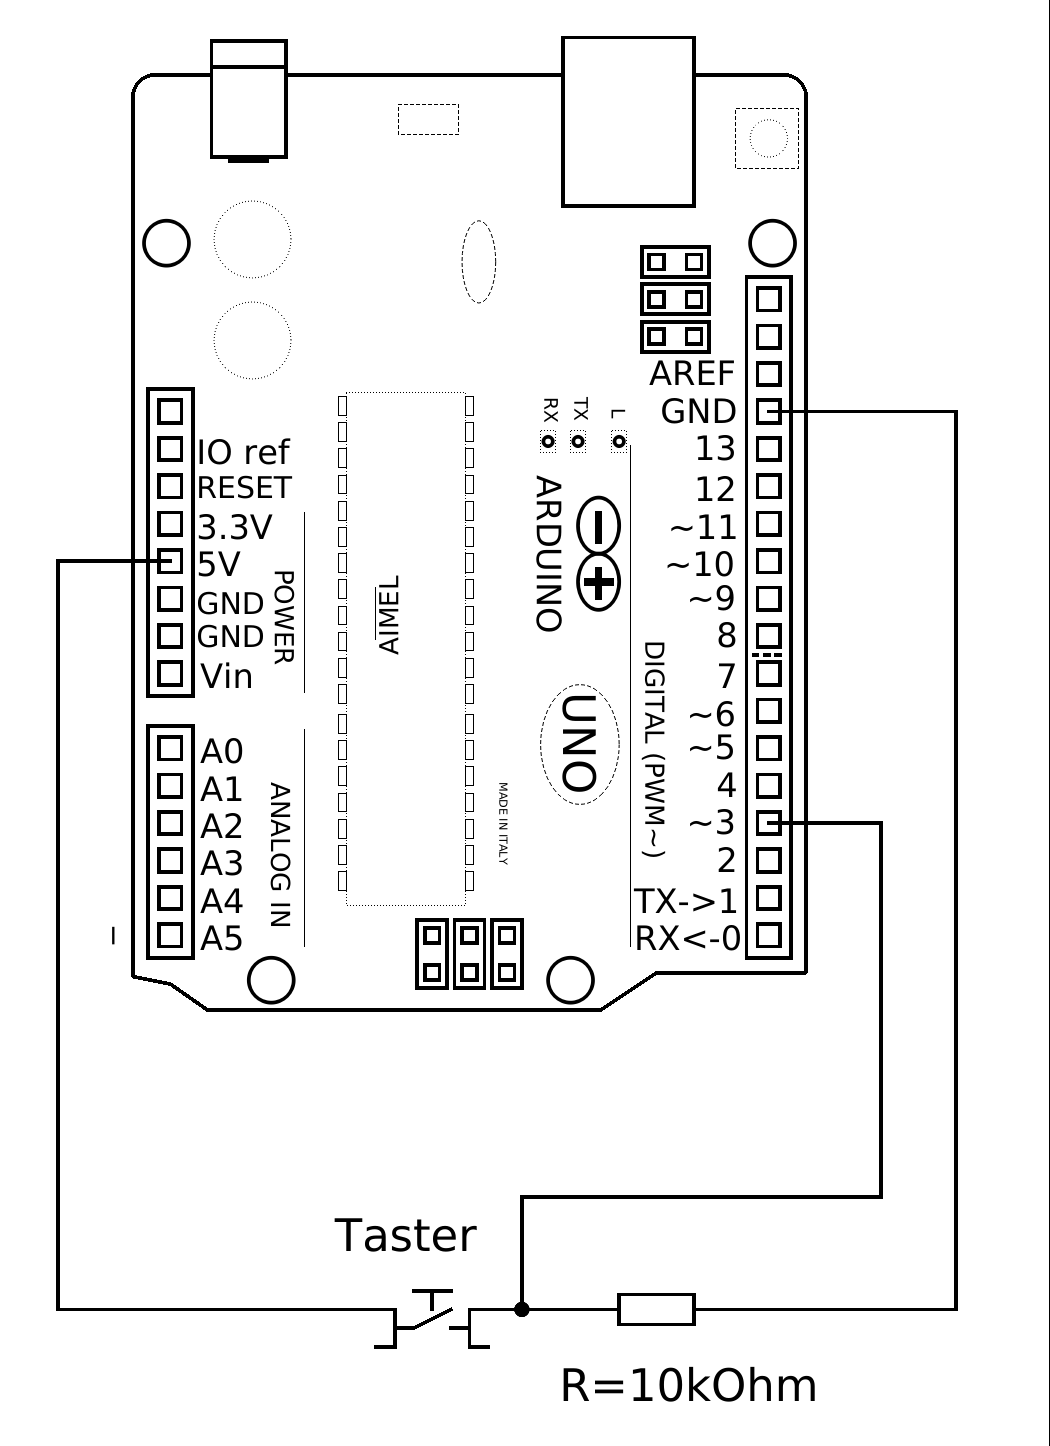
\includegraphics[width=0.8\textwidth]{./Zeichnungen/taster-an-arduino.png}
		\label{abb:schaltplan-taster}
	\end{figure}
\end{minipage}


\newpage
\begin{projekt}[Juke-Box]\label{proj:jukebox}
	\begin{wrapfigure}{r}{0.5\textwidth}
		\centering
		\vspace{-\baselineskip}
		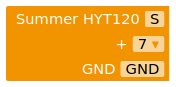
\includegraphics[width=0.25\textwidth]{pics/piezokonfiguration.png}
		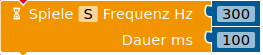
\includegraphics[width=0.35\textwidth]{pics/piezo-steuerung.png}
		\vspace{-\baselineskip}
		\label{abb:piezo-steuerung}
	\end{wrapfigure}
	Baue und programmiere eine Juke-Box!
	
	Die Juke-Box soll zwei verschiedene, kurze Melodien \emph{anspielen} können. Dazu werden zwei Taster auf die beschriebene Art an zwei digitale Pins des Arduino angeschlossen. Schließe zudem an einen Digitalpin einen Piezo-Summer an (siehe unten). 
	
	{\scriptsize Idee: Frick, Fritsch und Trick (2015): \emph{Einführung in Mikrocontroller - Der Arduino als Steuerzentrale}, Schülerforschungszentrum Bad Saulgau}
\end{projekt}

\emph{Hinweise:}

Zwei mögliche Beispiele von Melodien mit Link zu den Noten:
\begin{itemize}[itemsep=0ex, parsep=0mm]
	\item \href{https://www.lieder-archiv.de/alle\_meine\_entchen-notenblatt\_100055.html}{\enquote{Alle meine Entchen}}:
	
	\url{https://www.lieder-archiv.de/alle\_meine\_entchen-notenblatt\_100055.html},
	\item  \href{https://www.lieder-archiv.de/o\_tannenbaum-notenblatt\_200078.html}{\enquote{Oh Tannenbaum}}:
	
	\url{https://www.lieder-archiv.de/o\_tannenbaum-notenblatt\_200078.html}.
\end{itemize}

\emph{Frequenzen in Hertz zu den Noten:}

\begin{tabular}{c|c|c|c|c|c|c|c|c|c|c|c}\footnotesize
	$c^1$ & $cis^1/des^1$ & $d^1$ & $dis^1/es^1$ & $e^1$ & $f^1$ & $fis^1/ges^1$ & $g^1$ & $gis^1/as^1$ &  $a^1$ & $ais^1/b^1$ & $h^1$\\
	\hline \footnotesize
	 262 & 277 & 294 & 311 & 330 & 349 & 370 & 392 & 415 & 440 & 466 & 494\\
\end{tabular}

\medskip
\begin{zsfg}{Piezo-Summer}
	
	\begin{minipage}{0.7\textwidth}
		Mit einem Piezo-Summer lassen sich Töne erzeugen, wenn man eine Spannung anschließt. Das lange Bein muss dabei an den Pluspol (Pin) angeschlossen werden; das kurze an den Minuspol bzw. GND. Ein Vorwiderstand ist dabei nicht notwendig, hilft aber die Lautstärke zu reduzieren.
	\end{minipage}
	\hfill
	\begin{minipage}{0.28\textwidth}
		\begin{minipage}{0.48\textwidth}
			\centering
			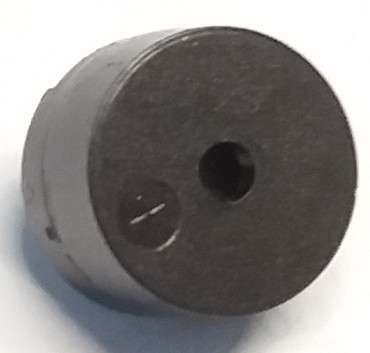
\includegraphics[width=0.9\textwidth]{./pics/piezo-summer.jpg}
		\end{minipage}
		\hfill
		\begin{minipage}{0.48\textwidth}
			\centering
			
\includegraphics[width=\textwidth]{./pics/piezo-schaltsymbol.png}
		\end{minipage}
	\end{minipage}
	
	\bigskip
	\emph{Funktionsweise:}\label{piezo-effekt}
	
	\begin{wrapfigure}{r}{0.4\textwidth}
		\vspace{-\baselineskip}
		\centering
		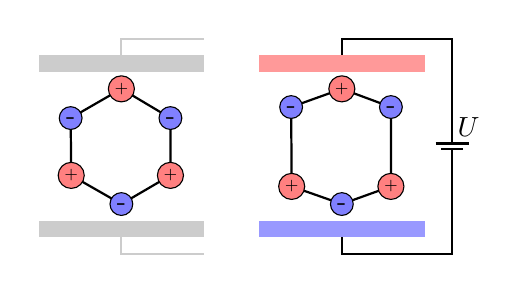
\begin{tikzpicture}[scale=0.7]
		\fill[white] (-0.2,-0.2) rectangle (8,4);
		%Kondensator links	
		\draw[gray!40,thick] (1.5,0.2) -- ++(0,-0.3) -- ++ (1.5,0);
		\fill[gray!40] (0,0.2) rectangle (3,0.5);
		\draw[gray!40,thick] (1.5,3.5) -- ++(0,0.3) -- ++ (1.5,0);
		\fill[gray!40] (0,3.2) rectangle (3,3.5);
		% Verbindungen/Sechseck
		\draw [thick] (1.5,0.8) -- (0.59,1.32) -- (0.58,2.36) -- (1.5,2.89) -- (2.39,2.36) -- (2.39,1.32) -- (1.5,0.8);
		%Ladungsverteilung
		\node at (1.5,0.8) [circle,fill=blue!50!white, draw, inner sep=1pt] (min1) {-};
		\node at (0.58,2.36) [circle,fill=blue!50!white, draw, inner sep=1pt] (min2) {-};
		\node at (2.39,2.36) [circle,fill=blue!50!white, draw, inner sep=1pt] (min3) {-};
		\node at (1.5,2.89) [circle,fill=red!50!white, draw, inner sep=1pt] (plus1) {\tiny +};
		\node at (0.59,1.32) [circle,fill=red!50!white, draw, inner sep=1pt] (plus2) {\tiny +};
		\node at (2.39,1.32) [circle,fill=red!50!white, draw, inner sep=1pt] (plus3) {\tiny +};
		%	
		%Kondensator rechts
		\draw[thick] (5.5,0.2) -- ++(0,-0.3) -- ++ (2,0) -- ++(0,1.9) ++(-0.2,0) -- ++(0.4,0);
		\fill[blue!40] (4,0.2) rectangle (7,0.5);
		\draw[thick] (5.5,3.5) -- ++(0,0.3) -- ++ (2,0) -- ++(0,-1.9) ++(-0.3,0) -- ++(0.6,0);
		\fill[red!40] (4,3.2) rectangle (7,3.5);
		\node at (7.8,2.2) {$U$};
		% Verbindungen/Sechseck rechts
		\draw [thick] (5.5,0.8) -- (4.59,1.12) -- (4.58,2.56) -- (5.5,2.89) -- (6.39,2.56) -- (6.39,1.12) -- (5.5,0.8);
		%Ladungsverteilung rechts
		\node at (5.5,0.8) [circle,fill=blue!50!white, draw, inner sep=1pt] (min11) {-};
		\node at (4.58,2.56) [circle,fill=blue!50!white, draw, inner sep=1pt] (min21) {-};
		\node at (6.39,2.56) [circle,fill=blue!50!white, draw, inner sep=1pt] (min31) {-};
		\node at (5.5,2.89) [circle,fill=red!50!white, draw, inner sep=1pt] (plus11) {\tiny +};
		\node at (4.59,1.12) [circle,fill=red!50!white, draw, inner sep=1pt] (plus21) {\tiny +};
		\node at (6.39,1.12) [circle,fill=red!50!white, draw, inner sep=1pt] (plus31) {\tiny +};
		\end{tikzpicture}
	\end{wrapfigure}
	In einem Piezo-Summer befindet sich ein Kristall mit unterschiedlichen Ladungsschwerpunkten, der von einem Kondensator umgeben ist. Wenn von außen an den Kristall eine Spannung angelegt wird, dann verformt sich die Kristallstruktur durch die Anziehung zwischen den Ladungsschwerpunkten und den Kondensatorplatten (\emph{\href{https://de.wikipedia.org/wiki/Piezoelektrizit\%C3\%A4t}{inverser piezo-elektrischer Effekt}}). Wenn keine Spannung anliegt, verformt sich der Kristall zurück. Durch diese Verformungen entstehen Druckwellen in der Luft, die wir als Ton wahrnehmen können.
\end{zsfg}

\section{Kommunikation mit dem Arduino: Der serielle Monitor}
\label{sec:seriellermonitor}

Bisher hatte die Kommunikation mit dem Arduino stets nur eine Richtung: Vom Computer zum Arduino. Das reicht nicht mehr, wenn eine Messung vorgenommen und deren Ergebnis zurück gemeldet werden soll. Die einfachste Möglichkeit, um dies zu realisieren, ist der serielle Monitor. Dieser soll im Folgenden genutzt werden, um eine Straßenlampe zu konfigurieren, die leuchtet, wenn es dunkel wird.

\begin{ziel}
	\textbf{Frage:} Wie kann der Arduino mit dem Computer kommunizieren?
\end{ziel}

\begin{aufgabe} \emph{Test des seriellen Monitors}
	
	\vspace{-0.5\baselineskip}
	\begin{enumerate}[label=\alph*), itemsep=0ex, parsep=0mm]
		\item Implementiere ein Programm, das in jeder Sekunde \enquote{Moin!} an den seriellen Monitor sendet und übertrage es auf den Arduino.
		
		\begin{figure}[H]
			\centering
			
\includegraphics[width=0.4\textwidth]{pics/serialprint.png}
		\end{figure}
		\vspace{-0.3\baselineskip}
		\item \href{https://jira.iais.fraunhofer.de/wiki/display/ORInfo/Vorbereitung+Nepo4Arduino#VorbereitungNepo4Arduino-SerialMonitor}{Öffne den seriellen Monitor} im Open Roberta Connector mit einer Baudrate von 9600 und kontrolliere dein Programm.
	\end{enumerate}
\end{aufgabe}

\bigskip
\begin{minipage}{0.48\textwidth}
	Ein LDR ist ein Widerstand, dessen Größe von der Lichtstärke abhängt, die auf ihn trifft (siehe unten). Um ihn auslesen zu können, muss er in einem sogenannten Spannungsteiler mit einem Festwiderstand von $R_1=\SI{10}{\kilo\ohm}$ an den Arduino angeschlossen werden (siehe rechts). Der zugehörige Konfigurationsblock ist unten abgebildet.
	
	\begin{minipage}{0.48\textwidth}
		\begin{figure}[H]
			\centering
			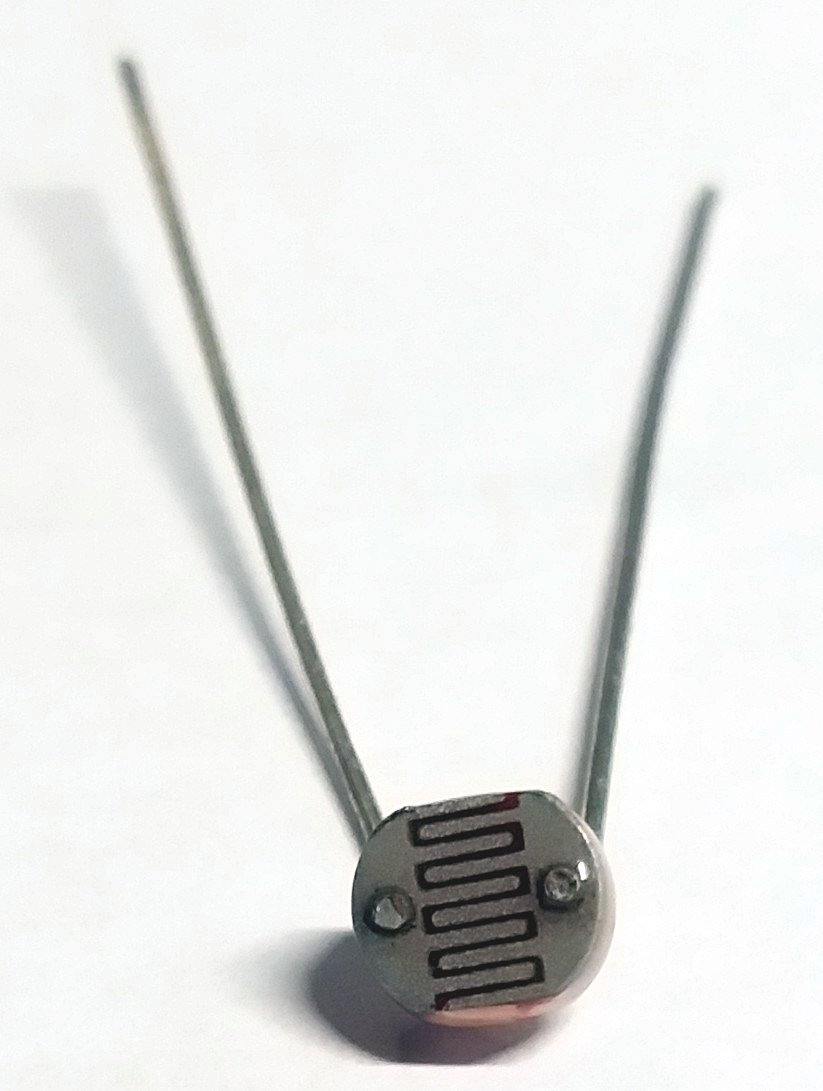
\includegraphics[width=0.5\textwidth]{./pics/ldr2.jpg}
			\caption{Ein LDR.}
		\end{figure}
	\end{minipage}
	\hfill
	\begin{minipage}{0.48\textwidth}
		\begin{figure}[H]
			\centering
			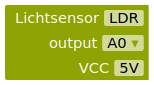
\includegraphics[width=0.9\textwidth]{./pics/ldr-konfiguration.png}
			\caption{Konfiguration des LDR.}
		\end{figure}
	\end{minipage}
\end{minipage}
\hfill
\begin{minipage}{0.48\textwidth}
	\begin{figure}[H]
		\centering
		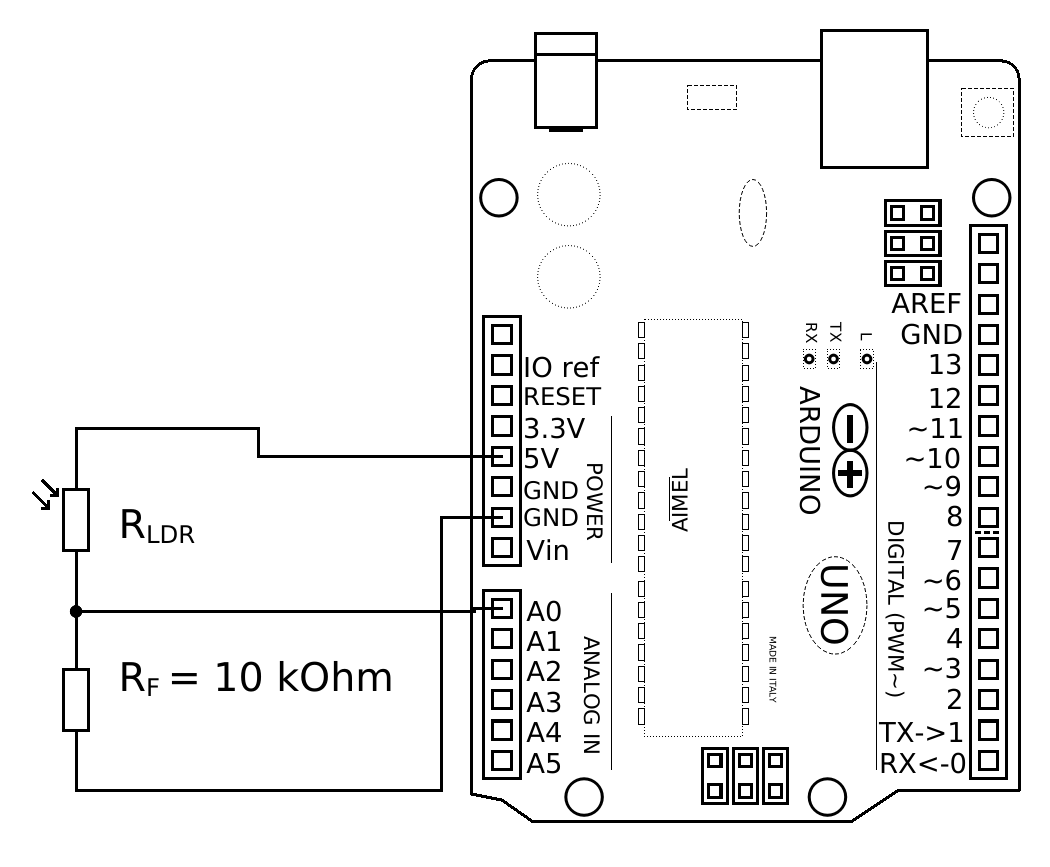
\includegraphics[width=\textwidth]{./Zeichnungen/ldr-an-arduino2.png}
		\label{abb:schaltplan-ldr}
	\end{figure}
\end{minipage}

\bigskip
\begin{aufgabe}\emph{Erste Experimente mit dem LDR}
	\vspace{-0.3\baselineskip}
	\begin{enumerate}[label=\alph*), itemsep=0ex, parsep=0mm]
		\item Baue die oben abgebildete Schaltung zum Auslesen eines LDR am Arduino auf und lasse dir die Lichtstärke in \% auf dem seriellen Monitor ausgeben.
		\item Die Veränderung der Lichtstärke in \% verläuft genau umgekehrt zur Veränderung des Widerstands des LDR. Beschreibe, wie sich der Widerstand des LDR verhält, wenn es dunkel bzw. wenn es hell wird.
	\end{enumerate}
\end{aufgabe}

\begin{projekt}[Straßenlampe]\label{proj:strassenlampe}
	Baue eine Straßenlampe, deren Licht (Vorwiderstand!) angeht, wenn es dunkel wird, und ausgeht, wenn es hell wird.
\end{projekt}

\begin{zsfg}{Fotowiderstand}
	\begin{minipage}{0.7\textwidth}
		Ein \textbf{Fotowiderstand}, kurz: \textbf{LDR} (\emph{engl. \textbf{l}ight \textbf{d}ependent \textbf{r}esistor}), ist ein lichtabhängiger Widerstand. Wenn es dunkel wird, wird der elektrische Widerstand des LDR größer; wenn es hell wird, wird der elektrische Widerstand des LDR kleiner.
	\end{minipage}
	\hfill
	\begin{minipage}{0.28\textwidth}
		\begin{minipage}{0.48\textwidth}
			\centering
			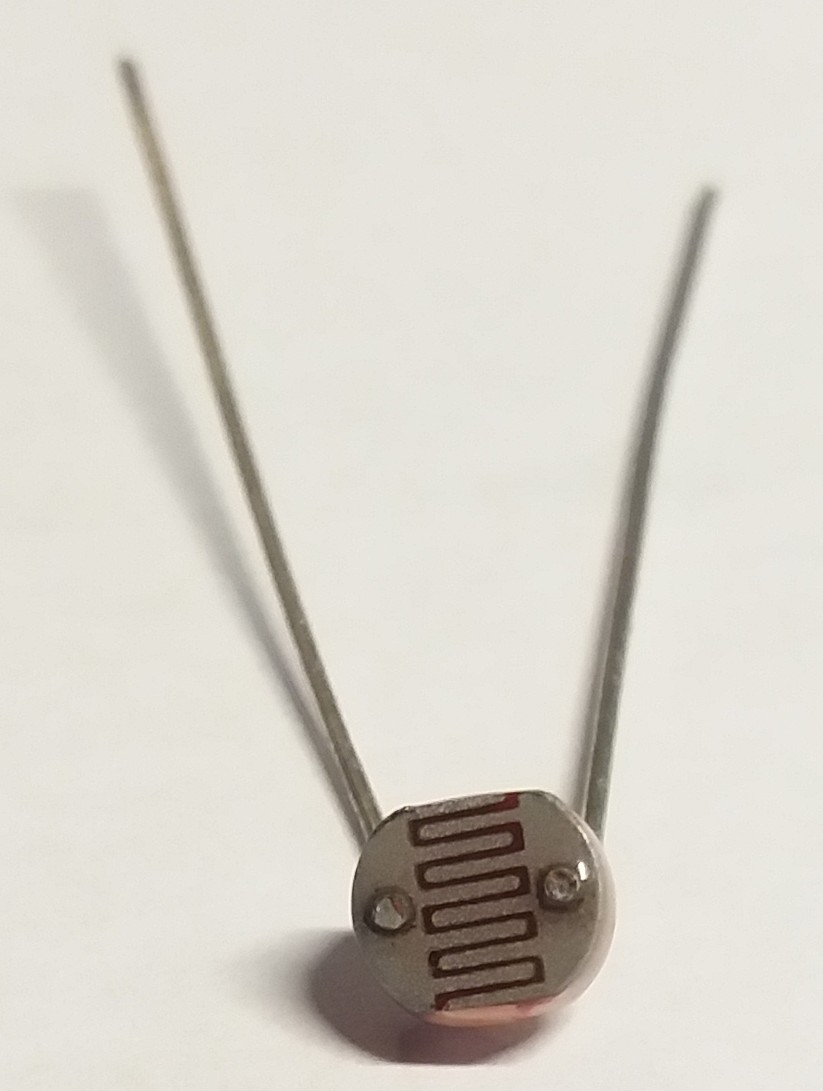
\includegraphics[width=0.9\textwidth]{./pics/ldr.jpg}
		\end{minipage}
		\hfill
		\begin{minipage}{0.48\textwidth}
			\centering
			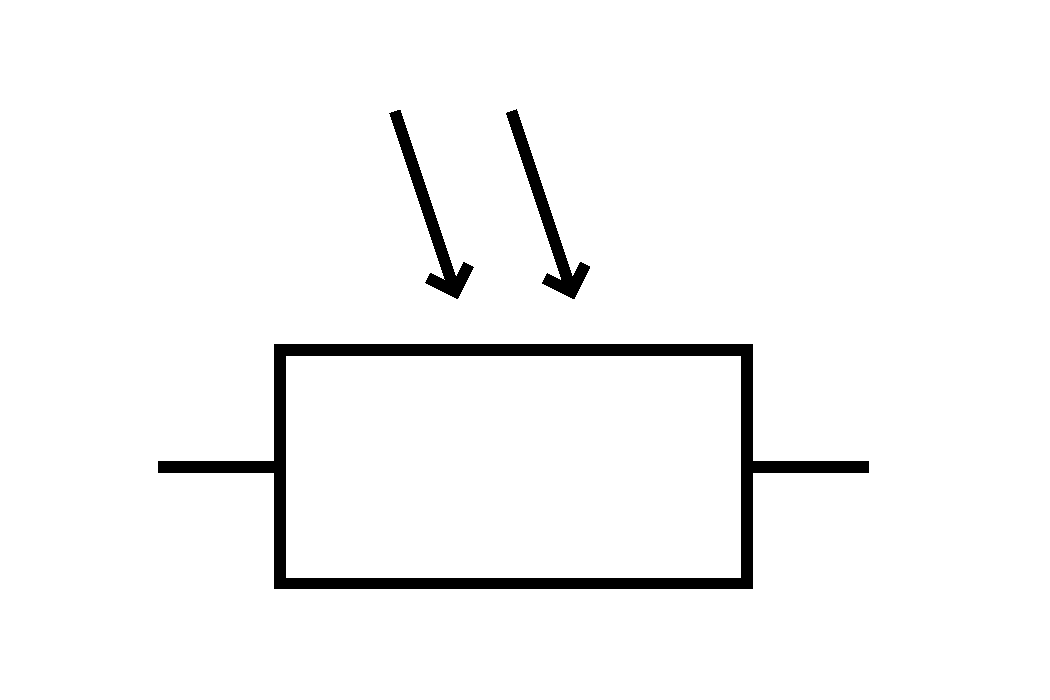
\includegraphics[width=\textwidth]{./pics/ldr-schaltsymbol.png}
		\end{minipage}
	\end{minipage}
	%	\bigskip
	%	\emph{Kurze Hintergrundinformation:}
	%	
	%	Der Fotowiderstand besteht aus einem Halbleitermaterial, in dem die Elektronen wie üblich an den Atomkern gebunden sind. Bei Halbleitern reicht jedoch schon relativ wenig Energie, um einige Elektronen so weit aus ihrer Bindung zu lösen, dass sie zum elektrischen Strom beitragen. Diese Energiezufuhr stammt von dem Licht, das auf den LDR fällt.
\end{zsfg}

\subsection{Reflexion: Datentypen}
\label{sec:datentypen}

\marginpar{%
	\textattachfile[description={Folie zu Kap. \thechapter, Datentypen}]{./Auftraege/kap3-auftrag-datentypen.pdf}{%
		\footnotesize\folie Folie %
	}%
	\footnotesize%
	\\öffnen%
}
\begin{aufgabe}
	\begin{enumerate}[label=\alph*), itemsep=0ex, parsep=0ex]
		\item In den bisherigen Anweisungen tauchten verschiedene Typen von Argumenten auf. Die Argumente sind unten noch einmal abgebildet. Gruppiere und charakterisiere sie.
		
		\bigskip
		\begin{tabu} to \textwidth {X[L]X[L,2]X[L,3]}
			
\includegraphics[width=0.1\textwidth]{./pics/zahlargument1.png} & 
			
\includegraphics[width=0.25\textwidth]{./pics/wahrheitswertargument1.png} & 
			
\includegraphics[width=0.38\textwidth]{./pics/zahlargument2.png} \\
			
\includegraphics[width=0.15\textwidth]{./pics/wahrheitswertargument2.png} & 
			
\includegraphics[width=0.2\textwidth]{./pics/textargument.png} & \\
		\end{tabu}
		\bigskip
		\item Begründe: Das Argument des \texttt{wenn}-Blocks muss hellblau sein. 
	\end{enumerate}
\end{aufgabe}

\bigskip
\begin{zsfg}{Datentypen}
	Alle Programmiersprachen unterscheiden verschiedene Datentypen, die unterschiedlich codiert sind. Die wichtigsten Datentypen in Nepo sind\dots
	\begin{itemize}
		\item 
\includegraphics[width=0.075\textwidth]{./pics/wahrheitswertargument2.png} logische Werte / Wahrheitswerte:
		
		Nur zwei Werte möglich, nämlich \texttt{wahr} oder \texttt{falsch},
		\item 
\includegraphics[width=0.05\textwidth]{./pics/zahlargument1.png} Zahlenwerte: 
		
		Sowohl ganze Zahlen als auch Dezimalzahlen (mit Punkt als Komma),
		\item 
\includegraphics[width=0.1\textwidth]{./pics/textargument.png} Zeichenketten: 
		
		Aneinanderreihung von Zeichen.
	\end{itemize}
\end{zsfg}

\vfill

\section{Entscheidungen mit mehreren Kriterien treffen}
\label{sec:wahrheitswerte}

Bisher waren die zu treffenden Entscheidungen immer nur von einem Kriterium abhängig. Das sind jedoch Ausnahmen. Nun geht es darum, wie man mehrere Kriterien miteinander kombinieren kann.

\begin{ziel}
	\textbf{Frage:} Wie lassen sich Entscheidungen mit mehreren Kriterien programmieren?
\end{ziel}

\begin{projekt}[Carport-Lampe]\label{proj:carportlampe}
	Baue und programmiere eine Carport-Lampe, die für einige Zeit leuchtet, wenn sie eine Bewegung registriert \tcbox[size=fbox,box align = base,colback=nepoLogik, colframe=gray,nobeforeafter]{\color{white}\bfseries\texttt{und}} es draußen gerade dunkel ist. In allen anderen Fällen bleibt die Lampe dunkel. Experimentiere mit den Drehreglern, um die Empfindlichkeit und Dauer des Signals richtig einzustellen.
\end{projekt}

\emph{Information zu Bewegungsmeldern:} Bewegungsmelder verfügen über drei Pins, deren Beschriftung man lesen kann, wenn man die Kunststofflinse vorsichtig abzieht (\emph{Vorsicht: Nach Abziehen der Linse nicht den Sensor berühren!}). \texttt{Vcc} und \texttt{GND} dienen der Stromversorgung der elektronischen Komponenten und müssen mit \texttt{5\,V} und \texttt{GND} am Arduino verbunden werden. 

Der mittlere \texttt{OUT}-Pin ist der Signal-Pin: Wenn eine Bewegung registriert wurde, wird der Wert \texttt{wahr} zurückgegeben, ansonsten \texttt{falsch}. Zum Einlesen des Signals wird dieser Pin mit einem Digitalpin des Arduino verbunden.

Hinten befinden sich zwei Drehregler (\enquote{Potentiometer}), mit denen sich die Dauer des Bewegungssignals (links) und die Empfindlichkeit (rechts) einstellen lassen. Zusätzlich befindet sich auf der rechten Seite ein sogenannter Jumper, mit dem auf einfache Weise eine Steckverbindung zwischen benachbarten Pins hergestellt werden kann. Wenn sich der Jumper ganz außen befindet, dann bleibt das Bewegungssignal nach dem Erkennen einer Bewegung eine Weile aktiv und wird dann auf jeden Fall deaktiviert. Eine neue Bewegung kann erst nach einer gewissen Zeit wieder registriert werden. Wenn der Jumper hingegen leicht nach innen versetzt ist, bleibt das Bewegungssignal so lange erhalten, wie eine Bewegung erkannt wird (siehe \href{https://funduino.de/nr-8-bewegungsmelder}{Funduino}).

\begin{minipage}{0.3\textwidth}
	\begin{figure}[H]
		\centering
		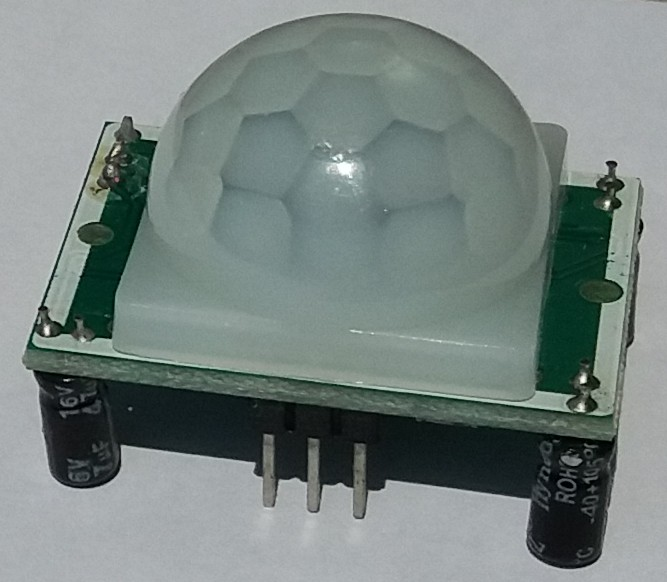
\includegraphics[width=0.67\textwidth]{pics/bewegungsmelder.jpg}
		\caption{Bewegungsmelder mit Linse.}
		\label{abb:bewegungsmelder}
	\end{figure}
\end{minipage}
\hfill
\begin{minipage}{0.3\textwidth}
	\begin{figure}[H]
		\centering
		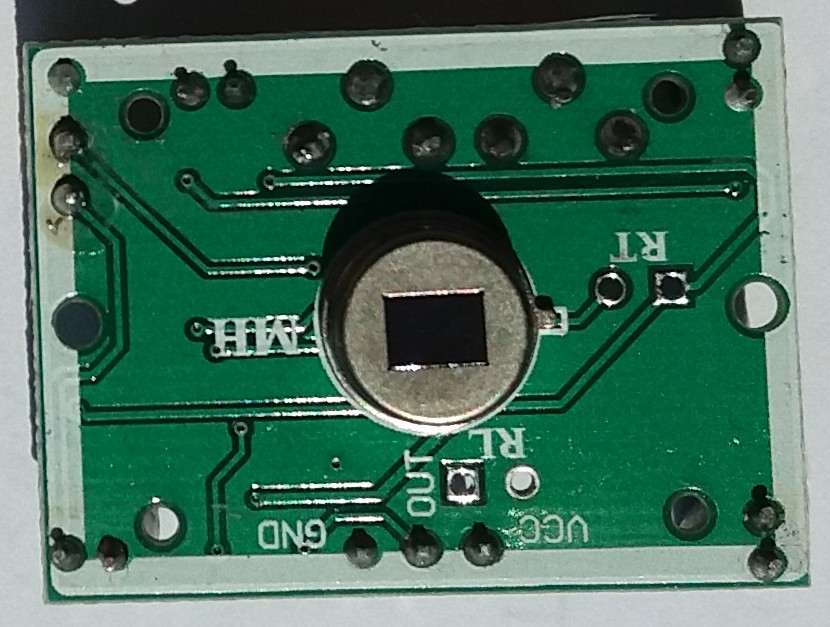
\includegraphics[width=0.83\textwidth]{pics/bewegungsmelder-ohne-linse.jpg}
		\caption{Pinbelegung.}
		\label{abb:bewegungsmelder-ohne-linse}
	\end{figure}
\end{minipage}
\hfill
\begin{minipage}{0.3\textwidth}
	\begin{figure}[H]
		\centering
		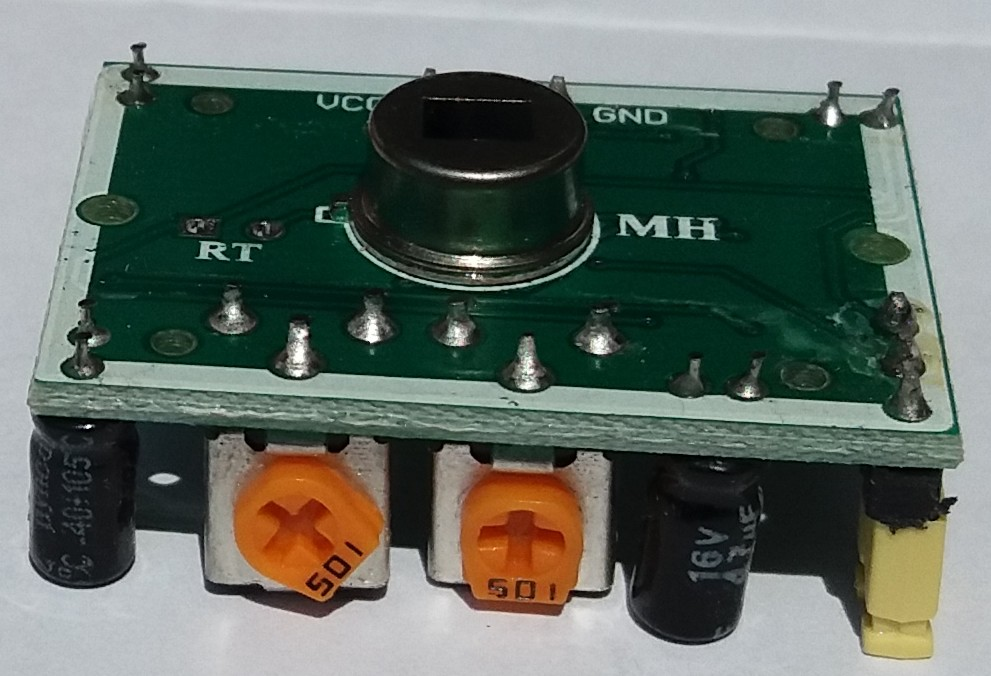
\includegraphics[width=0.83\textwidth]{pics/bewegungsmelder-hinten.jpg}
		\caption{Drehregler für Signaldauer (links) und Empfindlichkeit (rechts).}
		\label{abb:bewegungsmelder-hinten}
	\end{figure}
\end{minipage}

\vfill

\newpage
\begin{aufgabe} \emph{Wahrheitswerttabellen}
	\marginpar{%
		~\\
		~\\
		\footnotesize%
		\textattachfile[description={Arbeitsblatt zu Kap. \thechapter, Wahrheitswerttabellen}]{./Auftraege/kap3-ab-wahrheitswerttabellen.pdf}{
			\footnotesize%
			\drucker Arbeitsblatt%
		}
		\\öffnen%
	}
	\begin{enumerate}[label=\alph*), itemsep=0ex, parsep=0ex]
		\item Experimentiere mit der Carport-Lampe, um die folgende Wahrheitswert-Tabelle für die Operation UND auszufüllen.
		
			\medskip
			\begin{minipage}{0.4\textwidth}
				A: Bewegung registriert.
				
				B: Es ist dunkel.
			\end{minipage}
			\hfill
			\begin{minipage}{0.4\textwidth}
				\centering
				\begin{tabular}{c | c | c}
					\textbf{A} & \textbf{B} & \textbf{A UND B} \\ \hline
					wahr & wahr &  \\
					&  &  \\
					&  &  \\
					&  &  \\  
				\end{tabular}
			\end{minipage}
			\hfill
		
		\medskip
		\item Ändere das UND zu einem ODER und experimentiere wieder mit der Carport-Lampe, um die folgende Wahrheitswert-Tabelle für die Operation ODER auszufüllen.
		
			\medskip
			\begin{minipage}{0.4\textwidth}
				A: Bewegung registriert.
				
				B: Es ist dunkel.
			\end{minipage}
			\hfill
			\begin{minipage}{0.4\textwidth}
				\centering
				\begin{tabular}{c | c | c}
					\textbf{A} & \textbf{B} & \textbf{A ODER B} \\ \hline
					wahr & wahr &  \\
					&  &  \\
					&  &  \\
					&  &  \\  
				\end{tabular}
			\end{minipage}
			\hfill
		
		\medskip
		\item Ergänze die Wahrheitswerttabelle für die logische Operation NICHT.
			
			\medskip
			\begin{minipage}{0.4\textwidth}
				
			\end{minipage}
			\hfill
			\begin{minipage}{0.4\textwidth}
				\centering
				\begin{tabular}{c | c}
					\textbf{A}  & \textbf{NICHT A} \\ \hline
					wahr &  \\
					falsch &  \\  
				\end{tabular}
			\end{minipage}
			\hfill
	\end{enumerate}
\end{aufgabe}


\begin{zsfg}{Logische Operationen und Wahrheitswerttabellen}
	
	Logische Operationen dienen zum Verknüpfen von Wahrheitswerten - ganz so wie Rechenoperationen zum Verknüpfen von Zahlen dienen. Wir betrachten die logischen Operationen UND (AND), ODER (OR) sowie NICHT (NOT). Das Ergebnis dieser Operationen lässt sich anhand von Wahrheitswerttabellen übersichtlich festhalten. Darin wird festgehalten, ob zwei Aussagen bzw. Bedingungen A und B wahr (w) oder falsch (f) sind. In der rechten Spalte steht dann, ob die logische Operation wahr (w) oder falsch (f) ergibt.
	
	\medskip
	\begin{minipage}{0.3\textwidth}
		\centering
		\begin{tabular}{c | c | c}
			\textbf{A} & \textbf{B} & \textbf{A UND B} \\ \hline
			w & w & w \\
			w & f & f \\
			f & w & f \\
			f & f & f \\  
		\end{tabular}
	\end{minipage}
	\hfill
	\begin{minipage}{0.3\textwidth}
		\centering
		\begin{tabular}{c | c | c}
			\textbf{A} & \textbf{B} & \textbf{A ODER B} \\ \hline
			w & w & w \\
			w & f & w \\
			f & w & w \\
			f & f & f \\  
		\end{tabular}
	\end{minipage}
	\hfill
	\begin{minipage}[t]{0.3\textwidth}
		\centering
		\begin{tabular}{c | c}
			\textbf{A}  & \textbf{NICHT A} \\ \hline
			w & f \\
			f & w \\  
		\end{tabular}
	\end{minipage}
	
	\medskip
	Achtung: Die ODER-Operation ergibt auch dann \enquote{wahr}, wenn beide Aussagen wahr sind. Das aus dem Alltag bekannte \enquote{ENTWEDER-ODER} (XOR) ist eine weitere logische Operation, die \enquote{falsch} ergibt, wenn beide Aussagen wahr sind. Diese Operation ist aber nicht in Nepo enthalten.
\end{zsfg}

\begin{aufgabe} \emph{Verschachtelte Entscheidungen?!}
	
	Leo und Lara möchten ihre Carport-Lampe so umprogrammieren, dass sie nachts immer leuchtet und tagsüber nicht. Zusätzlich soll ein Alarm ertönen, wenn es Nacht ist und eine Bewegung registriert wird.
	
	Unten sind ihre Programme abgebildet. Entscheide jeweils (begründet!), ob das Programm für das geforderte Verhalten geeignet ist. Mache gegebenenfalls Verbesserungsvorschläge.
	
	\bigskip
	\begin{figure}[H]
		\begin{adjustwidth*}{-1.5cm}{-1.5cm}
			\centering
			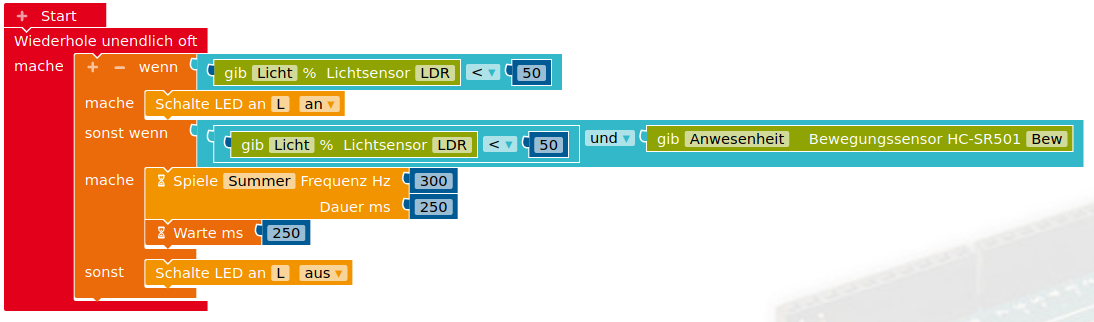
\includegraphics[width=1.2\textwidth]{./pics/wenn-sonstWenn-sonst-Bsp.png}
			\caption{Leos Programm.}
			\label{abb:sonstWenn1}
		\end{adjustwidth*}
	\end{figure}
	\begin{figure}[H]
		\begin{adjustwidth*}{-1.5cm}{-1.5cm}
			\centering
			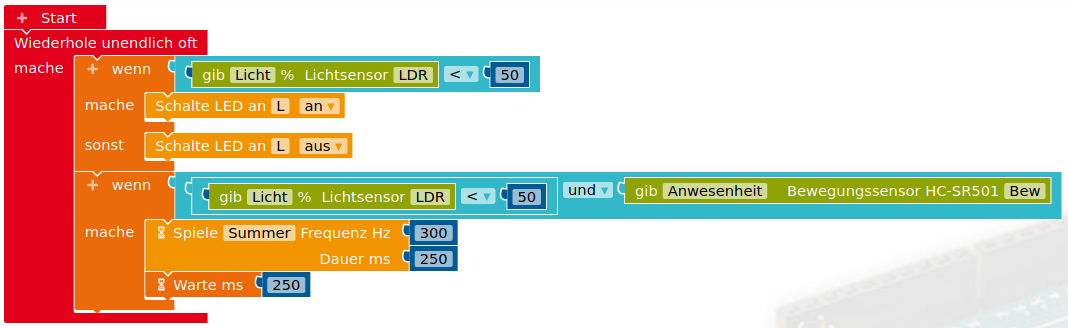
\includegraphics[width=1.2\textwidth]{./pics/wenn-sonstWenn-sonst-Bsp2.png}
			\caption{Laras Programm.}
		\end{adjustwidth*}
	\end{figure}
\end{aufgabe}

\newpage
\section{Programme mit Variablen und Schleifen effizient steuern}
\label{sec:variablenUndSchleifen}

\begin{aufgabe}
	Jana und Jonas haben jeweils LEDs an den Arduino angeschlossen und steuern diese mit den unten abgebildeten Programmen. Vergleiche die beiden Programme im Hinblick auf ihre Wirkung und die Art der Programmierung. Welches gefällt dir besser?
	
	Zusatzüberlegung: Wie viel muss man ändern, wenn man die Leuchtdauer ändern will?
\end{aufgabe}
\marginpar{%
	\textattachfile[description={Folie zu Kap. \thechapter, Variableneinsatz}]{./Auftraege/kap3-auftrag-variablen.pdf}{%
		\footnotesize\folie Folie %
	}%
	\footnotesize%
	\\öffnen%
}

\begin{figure}[H]
	\begin{minipage}{0.48\textwidth}
		\centering
		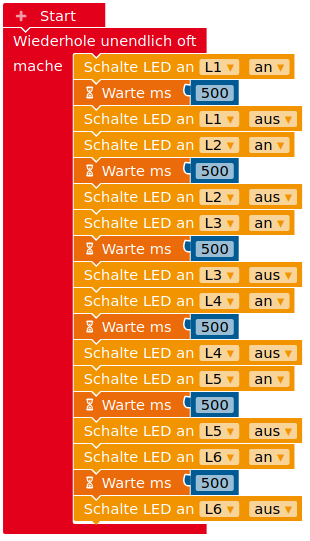
\includegraphics[width=0.8\textwidth]{./pics/lauflicht-ohne-variable.png}
		\caption{Janas Programm zum Steuern der LEDs.}
	\end{minipage}
	\hfill
	\begin{minipage}{0.48\textwidth}
		\centering
		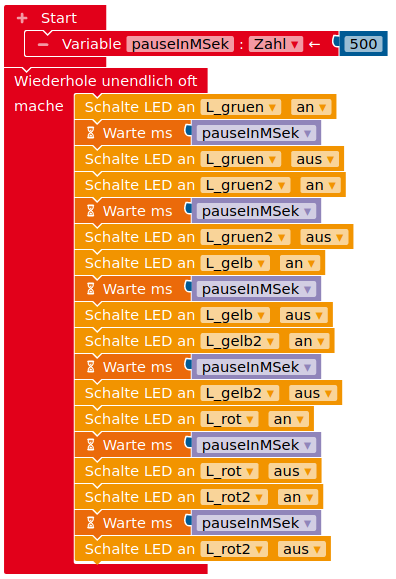
\includegraphics[width=\textwidth]{./pics/lauflicht-mit-variable.png}
		\caption{Jonas Programm zum Steuern der LEDs.}
	\end{minipage}
\end{figure}

\vspace{-0.5\baselineskip}
\begin{zsfg}{Variablen}
	\begin{wrapfigure}{r}{0.3\textwidth}
		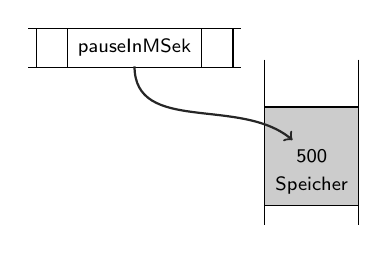
\begin{tikzpicture}[scale=0.5]
		\draw (-0.2,0) -- (5.2,0);
		\draw (-0.2,1) -- (5.2,1);
		\draw [fill=white] (0,0) rectangle (0.8,1);
		\draw [fill=white] (0.8,0) rectangle (4.2,1);
		\draw [fill=white] (4.2,0) rectangle (5,1);
		\node (pause) at (2.5,0.5) {\sffamily\scriptsize pauseInMSek};
		\draw (5.8,0.2) -- (5.8,-4);
		\draw (8.2,0.2) -- (8.2,-4);
		\draw [fill=gray!40] (5.8,-1) rectangle (8.2,-3.5);
		\node (wert) at (7,-2.25) {\sffamily\scriptsize 500};
		\draw [gray!30!black, thick,->] (pause) to [out=270,in=140] (wert);
		\node at (7,-3) {\sffamily\scriptsize Speicher};
		\end{tikzpicture}
	\end{wrapfigure}
	Eine Variable kann man sich als Koffer vorstellen, der einen Namen bekommt und in dem man einen festgelegten Datentyp speichert. Jedes Mal, wenn der Name des Koffers aufgerufen wird, wird der abgespeicherte Wert hervorgeholt und an die Stelle des Namens gesetzt. Intern wird der Variablenname als Verweis auf einen bestimmten Speicherplatz genutzt, in dem der Wert der Variable abgelegt ist.
	
	Für den Namen hat sich der \href{https://de.wikipedia.org/wiki/Binnenmajuskel#Programmiersprachen}{lowerCamelCase} etabliert: Der erste Buchstabe ist klein; wenn weitere Wörter folgen, fangen diese mit einem großen Buchstaben an. Leerzeichen sind nicht erlaubt.
\end{zsfg}

\subsection{Zufällige Ereignisse und Wiederholungen programmieren}


\begin{wrapfigure}{r}{0.4\textwidth}
	\quad \nepoexpert
	\begin{center}
		
\includegraphics[width=0.4\textwidth]{./pics/zufallszahl.png}
	\end{center}
\end{wrapfigure}
Viele Dinge werden interessanter, wenn sie sich nicht immer auf die genau gleiche Art wiederholen. Für diese Fälle kann man im Programm den blauen Block für Zufallszahlen verwenden (Expertenblöcke aktivieren!), der jedes Mal eine neue Zufallszahl erzeugt, wenn er aufgerufen wird. Ein einfaches Beispiel ist die \enquote{Bombe}, die man bei dem Spiel \enquote{Tick Tack Bumm} startet und die man so lange herum geben muss, bis sie explodiert. Dabei ist die Dauer des Tickens ein zufälliger Wert zwischen ca. 5\,s und 20\,s.
\marginpar{%
	\footnotesize%
	\video \\
	\href{https://el-voss.de/downloads/ticktack.html}{Bomben-Beispielvideo}
}

\bigskip
\begin{minipage}{0.73\textwidth}
	\begin{projekt}[Bombe bauen]\label{proj:bombe}
		Baue und programmiere eine \enquote{Bombe}, die für eine zufällige Dauer zwischen 5\,s und 20\,s tickt und dann explodiert. Die Bombe wird über einen Taster aktiviert.
		
		Zusatz: Welchen Unterschied macht es, wenn man die ausgewürfelte Zufallszahl in einer Variable speichert?
	\end{projekt}
\end{minipage}
\hfill
\begin{minipage}{0.25\textwidth}
	\centering
	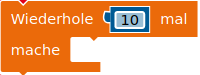
\includegraphics[width=0.8\textwidth]{./pics/wdh10mal.png}
\end{minipage}

\bigskip

\begin{aufgabe} \emph{Exkurs: Zufallszahlen von Mikrocontrollern/Mikroprozessoren}
	
	\begin{wrapfigure}{r}{0.7\textwidth}
		\centering
		\vspace{-0.5\baselineskip}
		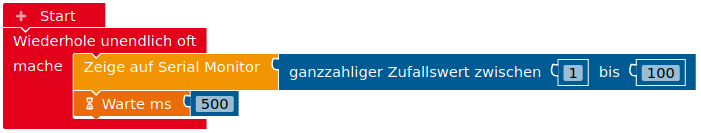
\includegraphics[width=0.7\textwidth]{./pics/zufallszahlengenerator.png}
	\end{wrapfigure}
	Übertrage das rechts abgebildete Programm auf den Arduino und betrachte die so erzeugten Zufallszahlen. Drücke dann auf den Reset-Taster am Arduino und betrachte die nun erzeugten Zufallszahlen. Wiederhole den Vorgang einige Male und beschreibe Auffälligkeiten.
\end{aufgabe}

%Reaktionszeitmesser mit Zufallselement; Aufgabe: Struktogramm

\bigskip
\begin{projekt}[Reaktionszeitmesser]\label{proj:reaktionszeitmesser}
	Baue und programmiere einen Reaktionszeitmesser.
	
	\begin{wrapfigure}{r}{0.3\textwidth}
		\centering
		
\includegraphics[width=0.28\textwidth]{./pics/stoppuhr2.png}
		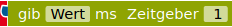
\includegraphics[width=0.28\textwidth]{./pics/stoppuhr.png}
	\end{wrapfigure}
	Der Reaktionszeitmesser soll zunächst warten, bis ein Taster gedrückt wurde, der besagt, dass es losgehen kann. Dann wird eine LED angeschaltet (Vorwiderstand!) und nach einer zufälligen Zeit wieder ausgeschaltet. Nun beginnt die Zeitmessung. Die Stoppuhr läuft solange, bis der Taster gedrückt wurde. Die gemessene Zeit wird dann über den seriellen Monitor ausgegeben und es wird erneut gewartet, bis der Anwender bestätigt, dass es losgehen kann.
	
	Miss mindestens zehn Mal deine Reaktionszeit und bestimme den Mittelwert. Bist du besser als dein Partner?
	
	{\scriptsize Idee: Frick, Fritsch und Trick (2015): \emph{Einführung in Mikrocontroller - Der Arduino als Steuerzentrale}, Bad Saulgau}
\end{projekt}

\subsection{Wiederholungen mit Bedingungen steuern}
\label{sec:while-schleife}

In vielen Fällen geht es bei Schleifen nicht um eine genau oder zufällig bestimmte Anzahl von Wiederholungen, sondern darum, einen Vorgang zu wiederholen, bis eine Bedingung wahr ergibt, bzw. solange, wie eine Bedingung wahr ergibt. Die Bedingung, die wahr oder falsch ergibt, kann auch Sensorwerte beinhalten. Dies wird auch im folgenden Spiel genutzt.

\bigskip
\begin{projekt}[Konfigurierbares Reaktionsspiel]\label{proj:reaktionsspiel}
	Baue und programmiere ein konfigurierbares Reaktionsspiel!
	
	\begin{wrapfigure}{r}{0.4\textwidth}
		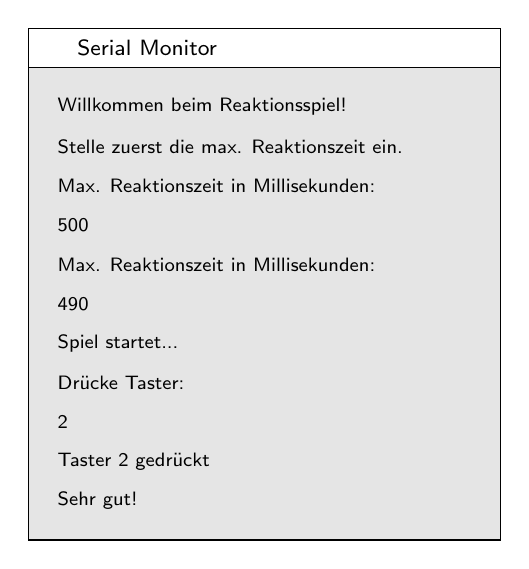
\begin{tikzpicture}
		\draw (0,6) rectangle (6,6.5) node at (0.5,6.25) [right] {\sffamily\footnotesize Serial Monitor};
		\draw [fill=gray!20] (0,0) rectangle (6,6);
		\node at (0.25,5.5) [right] {\sffamily\scriptsize Willkommen beim Reaktionsspiel!};
		\node at (0.25,5) [right] {\sffamily\scriptsize Stelle zuerst die max. Reaktionszeit ein.};
		\node at (0.25,4.5) [right] {\sffamily\scriptsize Max. Reaktionszeit in Millisekunden:};
		\node at (0.25,4) [right] {\sffamily\scriptsize 500};
		\node at (0.25,3.5) [right] {\sffamily\scriptsize Max. Reaktionszeit in Millisekunden:};
		\node at (0.25,3) [right] {\sffamily\scriptsize 490};
		\node at (0.25,2.5) [right] {\sffamily\scriptsize Spiel startet...};
		\node at (0.25,2) [right] {\sffamily\scriptsize Drücke Taster:};
		\node at (0.25,1.5) [right] {\sffamily\scriptsize 2};
		\node at (0.25,1) [right] {\sffamily\scriptsize Taster 2 gedrückt};
		\node at (0.25,0.5) [right] {\sffamily\scriptsize Sehr gut!};
		\end{tikzpicture}
	\end{wrapfigure}
	
	\medskip
	Dazu werden drei Taster (mit Widerstand!) am Arduino angeschlossen. Nach einer zufälligen Zeit wird auf dem seriellen Monitor angezeigt, welcher (zufällig ausgewürfelte) Taster gedrückt werden soll. Geschieht dies innerhalb einer vorgegebenen maximalen Reaktionszeit, hat man gewonnen, andernfalls verloren.
	
	Am Anfang des Spiels soll diese maximale Reaktionszeit konfiguriert werden können. Das heißt, man kann die max. Reaktionszeit mit dem linken Taster verringern und mit dem rechten Taster vergrößern. Erst wenn der mittlere Taster gedrückt wird, startet das Spiel.
	
	\medskip
	Für einen besseren Zugang zu diesem komplexen Spiel kannst du folgende Vorlage öffnen, mittels \enquote{Speichern unter} als \texttt{Reaktionsspiel.xml} auf dem Computer speichern und die Datei im Open Roberta Lab importieren:
	\textattachfile[mimetype=text/plain, description={Vorlage zur Programmierung eines frei konfigurierbaren Reaktionsspiels}]{./lsg/NEPO-Reaktionsspiel-Start.xml}{
		reaktionsspiel-vorlage.xml%
	}.
\end{projekt}

\emph{Mögliche Erweiterungen:}
\begin{itemize}[itemsep=0ex, parsep=0ex]
	\item zusätzliche Ausgabe der Reaktionszeit,
	\item Ober- und Untergrenze für die einstellbare maximale Reaktionszeit, damit das Spiel nicht unmöglich, aber auch nicht zu langweilig wird,
	\item nach Spielstart folgen mehrere Spiele hintereinander und es wird mitgezählt, wie oft gewonnen wird,
	\item je nach Reaktionszeit bekommt man mehr oder weniger Punkte,
	\item \dots
\end{itemize}

\newpage
\subsection{Zählschleifen programmieren}
\label{sec:for-schleife}

Lauflichter findet man inzwischen überall in unserer Welt: An den Rändern von Landebahnen an Flughäfen, an Spieleautomaten, aufdringlichen Werbeschildern, als Blinker von modernen Autos und vieles mehr. Wenn man diese programmieren will, eignen sich dazu am besten Zählschleifen.

\medskip
\begin{aufgabe} \emph{Zählschleifen verstehen}
	
	\begin{wrapfigure}{r}{0.7\textwidth}
		\centering
		\vspace{-0.5\baselineskip}
		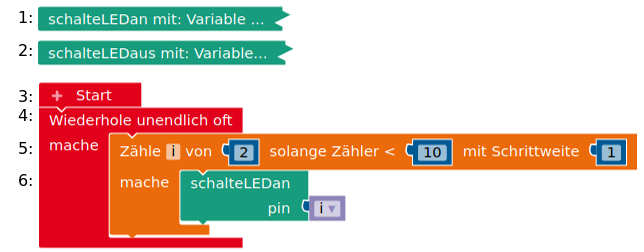
\includegraphics[width=0.68\textwidth]{./pics/for-schleife-bsp.png}
	\end{wrapfigure}
	Das rechts abgebildete Programm enthält zwei selbst definierte Blöcke, mit denen sich eine LED an einem beliebigen Pin zwischen 2 und 13 anstellen bzw. ausschalten lässt. In der Endlosschleife wird dann eine Zählschleife genutzt.
	
	\medskip
	Stelle eine Vermutung an, was die Zählschleife bewirkt.
	
	\medskip
	Überprüfe deine Vermutung mit Hilfe einer \emph{Trace-Tabelle} (siehe unten).
\end{aufgabe}

\begin{zsfg}{Trace-Tabellen}
	\begin{minipage}{0.78\textwidth}
		Trace-Tabellen stellen den Wert von Variablen beim Durchlaufen des Programms dar. Auf diese Art und Weise kann man sich zum Beispiel genau veranschaulichen, wann Schleifen abgebrochen werden.
	\end{minipage}
	\hfill
	\begin{minipage}{0.2\textwidth}
		\centering
		\scriptsize
		\begin{tabular}{l | c}
			\textbf{Zeile} & \textbf{i} \\ \hline
			\dots & \dots \\ \hline
			5 & 2 \\ \hline
			6 & 2 \\ \hline
			5 & 3 \\ \hline
			6 & 3 \\ \hline
		\end{tabular}
	\end{minipage}	
\end{zsfg}

\bigskip
\marginpar{%
	\footnotesize%
	\video \\
	\href{https://www.youtube.com/watch?v=s317_5aFL6E}{Blinker-Beispielvideo}
}
\begin{projekt}[Auto-Blinker]\label{proj:blinker}
	Programmiere ein Lauflicht so, wie es auch als Blinker in modernen Autos genutzt wird. Nutze zunächst nur 5 LEDs (mit Vorwiderstand!).
	
	\medskip
	\emph{Hinweis:} Du kannst das folgende Programm als Vorlage nutzen, damit du auch über die selbst definierten Blöcke zum Anstellen bzw. Ausstellen einer LED an einem beliebigen Pin zwischen 2 und 13 verfügst. Öffne das Programm, speichere es als \texttt{blinker.xml} und importiere es in Open Roberta Lab:
	\textattachfile[mimetype=text/plain, description={Vorlage zur Programmierung eines Lauflichtes}]{./lsg/NEPO-lauflicht-start.xml}{
		blinker-vorlage.xml%
	}.
\end{projekt}

\begin{aufgabe} \emph{La - o - La}
	
	Programmiere ein Lauflicht, das hin- und zurückläuft.
\end{aufgabe}

\vfill

\begin{aufgabe} \emph{Steuerung von Schleifen}
	
	Unten siehst du zwei Programme, für die jeweils fünf LEDs mit Vorwiderstand an Pin 2 bis 6 angeschlossen wurden. Baue das nach, importiere die Programme in Open Roberta Lab und übertrage sie auf den Arduino.
	
	Beschreibe die Wirkung von \texttt{Die Schleife abbrechen} und \texttt{mit der nächsten Iteration der Schleife fortfahren}.
	
	\bigskip
	\begin{minipage}{0.48\textwidth}
		\centering
		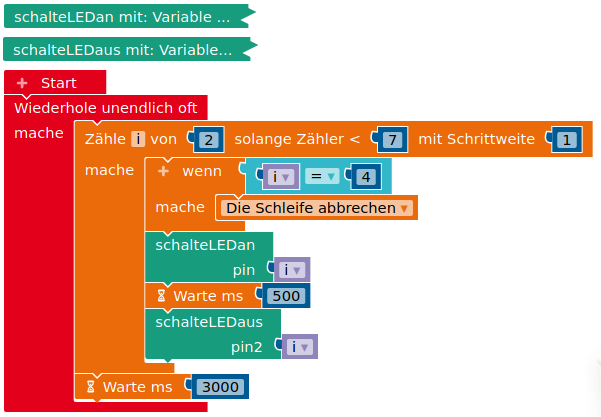
\includegraphics[width=\linewidth]{./pics/break-bsp.png}
		\bigskip
		\textattachfile[mimetype=text/plain, description={Vorlage zur Untersuchung eines Schleifenabbruchs}]{./lsg/NEPO-break-Bsp.xml}{
			schleife-abbrechen.xml%
		}
	\end{minipage}
	\hfill
	\begin{minipage}{0.48\textwidth}
		\centering
		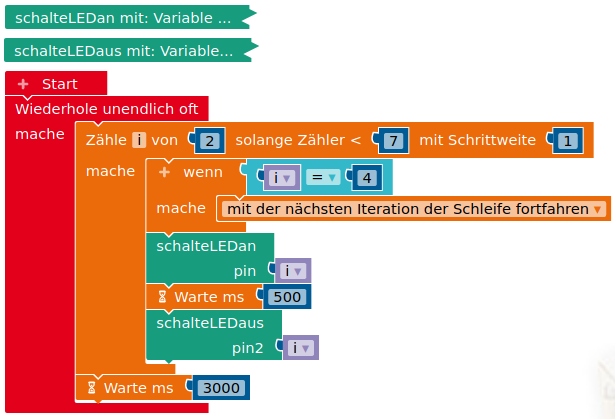
\includegraphics[width=\linewidth]{./pics/continue-bsp.png}
		\bigskip
		\textattachfile[mimetype=text/plain, description={Vorlage zur Untersuchung eines Schleifensprungs}]{./lsg/NEPO-continue-Bsp.xml}{
			schleife-fortfahren.xml%
		}
	\end{minipage}
\end{aufgabe}

\bigskip
In Nepo wie in anderen Programmiersprachen gibt es verschiedene Arten von Schleifen. Bisher wurde in Nepo die einfache Zählschleife \texttt{wiederhole x mal}, die bedingungsgesteuerte Wiederholschleife \texttt{wiederhole bis / solange} und die Zählschleife mit Zählervariable genutzt. Tatsächlich lässt sich das gleiche Verhalten aber mit allen drei Schleifenvarianten erreichen.

\begin{aufgabe} \emph{Vergleich von Schleifen}
	
	Betrachte noch einmal das Programm \texttt{schleife-abbrechen.xml} (siehe oben). Implementiere das gleiche Verhalten mit \dots
	\begin{enumerate}[label=\alph*), itemsep=0ex, parsep=0ex]
		\item \dots einer \texttt{wiederhole x mal} Schleife,
		\item \dots einer \texttt{wiederhole bis} Schleife,
		\item \dots einer \texttt{wiederhole solange} Schleife.
	\end{enumerate}

	Erkläre, welche Schleifenvariante sich als \enquote{Grundschleife} eignet, die die anderen Varianten \emph{immer} ersetzen kann.
\end{aufgabe}

\newpage
\begin{zsfg}{Sichtbarkeit: Lokale und globale Variablen}
	Ein Unterschied zwischen den Schleifenimplementierungen bleibt bestehen: Die Zählvariable \texttt{i} wird bei einer Zählschleife als \emph{lokale Variable} angelegt, das heißt, man kann die Zählvariable nur \emph{innerhalb der Schleife} nutzen. Dafür benötigt sie auch nur innerhalb der Schleife Speicherplatz.
	
	Im Gegensatz dazu sind die unter \texttt{Start} angelegten Variablen überall im Programm bzw. global verfügbar und heißen deshalb \emph{globale Variablen}. Für diese Variablen muss während der ganzen Zeit Speicherplatz bereitgehalten werden, auch wenn sie vielleicht nur an einer Stelle wirklich benötigt werden.
\end{zsfg}

\begin{zsfg}{Schleifen}
	
	Bei der Programmierung werden häufig Schleifen genutzt, die die Anweisungen in ihrem Rumpf (oder Körper) solange wiederholen, bis eine gewisse Abbruchbedingung eintritt.
	
	\begin{itemize}[itemsep=0ex, parsep=0ex]
		\item \texttt{wiederhole x mal}: Einfache \emph{Zählschleife}, die die Anweisungen im Rumpf für eine festgelegte Anzahl wiederholt.
		\item \texttt{wiederhole, bis}: Bedingungsgesteuerte Schleife, die die Anweisungen im Rumpf wiederholt, \emph{bis} die Bedingung wahr ergibt.
		\item \texttt{wiederhole, solange}: Bedingungsgesteuerte Schleife, die die Anweisungen im Rumpf wiederholt, \emph{solange} die Bedingung wahr ergibt.
		\item \texttt{zähle i von \dots ~solange Zähler \dots ~mit Schrittweite \dots}: Zählergesteuerte Schleife, die die Anweisungen im Rumpf wiederholt, solange der Zähler kleiner als eine vorgegebene Zahl ist und die Zählervariable nach jedem Durchlauf um eine angegebene Zahl erhöht.
	\end{itemize}
		
	Die Überprüfung, ob die Bedingung wahr ist, erfolgt hier \emph{vor} der Ausführung der Anweisungen im Rumpf. Daher nennt man die Schleifen auch \emph{kopfgesteuert}.
\end{zsfg}


\newpage
\section{Programme mit Struktogrammen dokumentieren}
\label{sec:struktogramme}

Wenn wir uns über Programme austauschen, dann haben wir nicht immer den Computer zur Hand. In solchen Momenten wäre es viel zu aufwendig, die bunten Blöcke von Nepo zu malen. Außerdem könnte es sein, dass jemand anderes das Programm nicht mit Blöcken, sondern mit Text in der Programmiersprache C++ aufschreiben will, also so wie der ~\nepoquellcode Quellcode aussieht.

\begin{ziel}
	\textbf{Frage:} Wie kann man Programme übersichtlich zu Papier bringen?
\end{ziel}

Man nutzt zur Darstellung des Ablaufs eines Computerprogramms sogenannte \textbf{Struktogramme} (vgl. Tab. \ref{tab:struktogramm}), die in den 1970er Jahren von Isaac Nassi und Ben Shneidermann entwickelt wurden. Struktogramme sollen ein Computerprogramm möglichst einfach und ohne programmiersprachenspezifische Befehlssyntax abbilden. Auf diese Art und Weise lassen sich Programme auch einfach planen, bevor man sich damit beschäftigt, wie die Schritte im Einzelnen zu codieren sind.

\begin{aufgabe}
	Stelle die unten abgebildeten Programme jeweils mithilfe eines Struktogramms dar.
\end{aufgabe}

\begin{figure}[H]
	\begin{adjustwidth}{-1.5cm}{1.5cm}
		\centering
		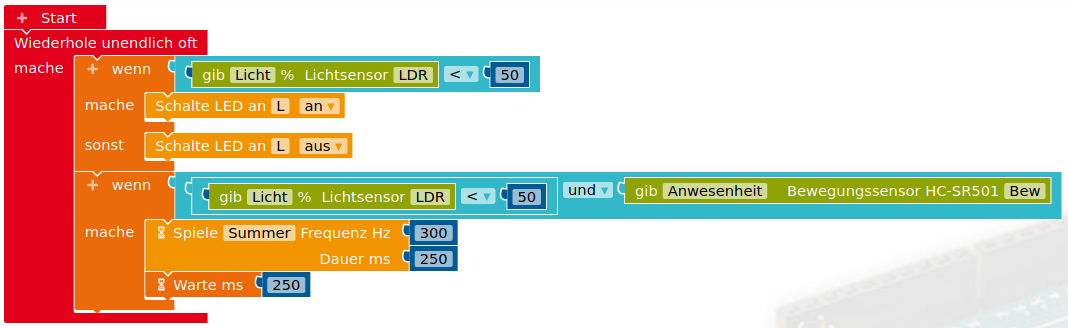
\includegraphics[width=1.2\textwidth]{./pics/wenn-sonstWenn-sonst-Bsp2.png}
		\caption{Programm A.}
	\end{adjustwidth}
\end{figure}
%\vspace{-\baselineskip}
\begin{figure}[H]
	\centering
	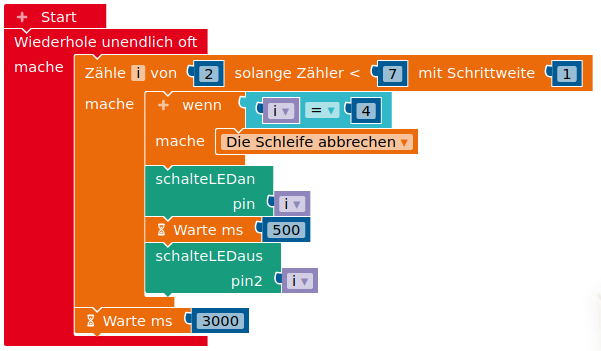
\includegraphics[width=0.7\textwidth]{./pics/break-bsp-schmal.png}
	\caption{Programm B.}
\end{figure}

\newpage

\begin{zsfg}{Darstellung von Programmen in Struktogrammen}
	
	\begin{table}[H]
		\centering
		\begin{minipage}[b]{\textwidth}
			\begin{tabu} to \textwidth {X[L,3]X[L,2]}
				\toprule
				\vspace{-4\baselineskip}
				\textbf{Lineare Struktur}
				
				Jede Anweisung wird in einen rechteckigen Block geschrieben.
				
				&
				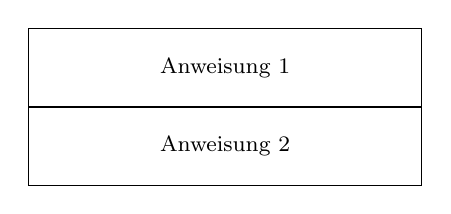
\begin{tikzpicture}
				\draw (0,0) rectangle (5,1);
				\node at (2.5,0.5) {\footnotesize Anweisung 2};
				\draw (0,1) rectangle (5,2);
				\node at (2.5,1.5) {\footnotesize Anweisung 1};
				\end{tikzpicture}
				\\
				\midrule%\hline
				%\rowcolor{CadetBlue!80!green}
				\textbf{Wiederholung / Schleifen} & \\
				\midrule%\hline
				%         \vspace{-4.2\baselineskip}
				\vspace{0mm}
				\textbf{Zählergesteuerte Schleife}
				
				Die Anzahl der Schleifendurchläufe wird durch eine Zählvariable festgelegt. Im Schleifenkopf werden der Startwert der Zählvariablen, der Endwert der Zählvariablen und die Veränderung der Zählvariablen, z.\,B. Schrittweite 1, angegeben.
				&
				\smallbreak
				\vspace{-0.7\baselineskip}
				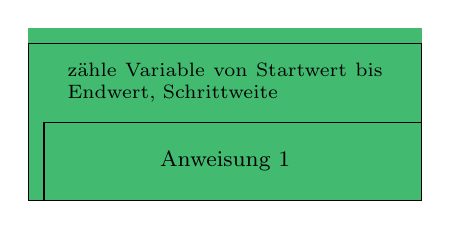
\begin{tikzpicture}
				\fill [CadetBlue!70!green] (0,0) rectangle (5,2.2);
				\draw (0,0) -- (0,2) -- (5,2) -- (5,1) -- (0.2,1) -- (0.2,0) -- (0,0);
				\draw (0.2,0) -- (5,0) -- (5,1);
				\node at (2.5,0.5) {\footnotesize Anweisung 1};
				\node at (2.5,1.5) {\parbox{4cm}{\scriptsize zähle Variable von Startwert bis Endwert, Schrittweite}};
				\end{tikzpicture}
				\\
				\midrule
				\vspace{-4\baselineskip}
				\textbf{Kopfgesteuerte Schleife}
				
				Wiederholungsschleife mit vorausgehender Prüfung der Bedingung. Der Schleifenkörper wird so lange wiederholt, \emph{wie} oder \emph{bis} die Bedingung wahr ist (bei uns nur der letzte Fall verfügbar).
				&
				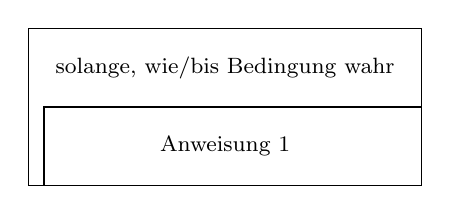
\begin{tikzpicture}
				\draw (0,0) -- (0,2) -- (5,2) -- (5,1) -- (0.2,1) -- (0.2,0) -- (0,0);
				\draw (0.2,0) -- (5,0) -- (5,1);
				\node at (2.5,0.5) {\footnotesize Anweisung 1};
				\node at (2.5,1.5) {\footnotesize solange, wie/bis Bedingung wahr};
				\end{tikzpicture}
				\\
				\midrule
				\vspace{-4\baselineskip}
				\textbf{Fußgesteuerte Schleife}
				
				Wiederholungsschleife mit nachfolgender Prüfung der Bedingung. Der Schleifenkörper wird so lange wiederholt, \emph{wie} oder \emph{bis} die Bedingung wahr ist (in mBlock nicht verfügbar).\smallskip
				&
				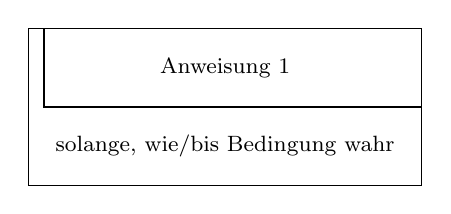
\begin{tikzpicture}
				\draw (0,0) -- (0,2) -- (0.2,2) -- (0.2,1) -- (5,1) -- (5,0) -- (0,0);
				\draw (0.2,2) -- (5,2) -- (5,1);
				\node at (2.5,1.5) {\footnotesize Anweisung 1};
				\node at (2.5,0.5) {\footnotesize solange, wie/bis Bedingung wahr};
				\end{tikzpicture}
				\\
				\midrule%\hline
				%\rowcolor{CadetBlue!80!green}
				\textbf{Verzweigung} & \\
				\midrule%\hline
				\vspace{0mm}
				\textbf{Einfache Verzweigung}
				
				Die Anweisung 1 (und ggf. weitere) wird nur ausgeführt, falls die Bedingung wahr ist. Andernfalls wird nichts gemacht.
				&
				\smallbreak
				\vspace{-0.7\baselineskip}
				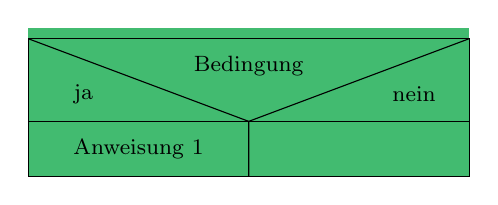
\begin{tikzpicture}[scale=0.7]
				\fill [CadetBlue!70!green] (0,0) rectangle (8,2.7);
				\draw (0,0) rectangle (8,2.5);
				\draw (0,1) -- (8,1);
				\draw (4,0) -- (4,1) -- (8,2.5);
				\draw (4,1) -- (0,2.5);
				\node at (2,0.5) {\footnotesize Anweisung 1};
				\node at (1,1.5) {\footnotesize ja};
				\node at (7,1.5) {\footnotesize nein};
				\node at (4,2) {\footnotesize Bedingung};
				\end{tikzpicture}
				\\
				\midrule
				\vspace{-3.5\baselineskip}
				\textbf{Alternative Verzweigung}
				
				Falls die Bedingung wahr ist, wird Anweisung 1 (und ggf. weitere) ausgeführt, sonst wird Anweisung 2 (und ggf. weitere) ausgeführt.
				&
				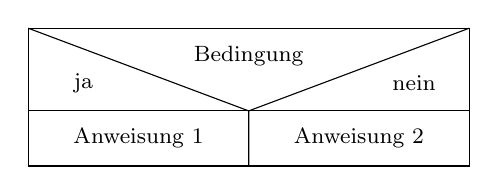
\begin{tikzpicture}[scale=0.7]
				\draw (0,0) rectangle (8,2.5);
				\draw (0,1) -- (8,1);
				\draw (4,0) -- (4,1) -- (8,2.5);
				\draw (4,1) -- (0,2.5);
				\node at (2,0.5) {\footnotesize Anweisung 1};
				\node at (6,0.5) {\footnotesize Anweisung 2};
				\node at (1,1.5) {\footnotesize ja};
				\node at (7,1.5) {\footnotesize nein};
				\node at (4,2) {\footnotesize Bedingung};
				\end{tikzpicture}
				\\
				\midrule
				\vspace{-5.5\baselineskip}
				\textbf{Verschachtelte Verzweigung}
				
				Falls Bedingung 1 wahr ist, folgt eine weitere Bedingung 2.
				&
				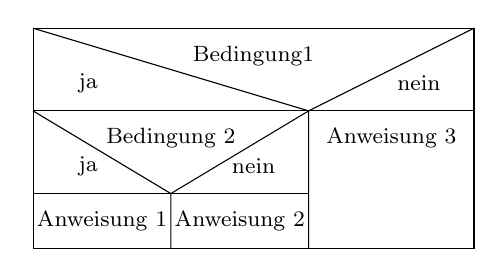
\begin{tikzpicture}[scale=0.7]
				\draw (0,-1.5) rectangle (8,2.5);
				\draw (0,1) -- (8,1);
				\draw (5,-1.5) -- (5,1) -- (8,2.5);
				\draw (5,1) -- (0,2.5);
				\draw (2.5,-1.5) -- (2.5,-0.5) -- (5,1);
				\draw (0,1) -- (2.5,-0.5);
				\draw (0,-0.5) -- (5,-0.5);
				\node at (1,1.5) {\footnotesize ja};
				\node at (7,1.5) {\footnotesize nein};
				\node at (4,2) {\footnotesize Bedingung1};
				\node at (1,0) {\footnotesize ja};
				\node at (4,0) {\footnotesize nein};
				\node at (2.5,0.5) {\footnotesize Bedingung 2};
				\node at (1.25,-1) {\footnotesize Anweisung 1};
				\node at (3.75,-1) {\footnotesize Anweisung 2};
				\node at (6.5,0.5) {\footnotesize Anweisung 3};
				\end{tikzpicture}
				\\
				\bottomrule
			\end{tabu}
		\end{minipage}
		\caption{Tabelle zur Darstellung eines Programms als Struktogramm nach Nassi und Shneidermann.}
		\label{tab:struktogramm}
	\end{table}
	
\end{zsfg}

\section{Eigene Funktionen definieren}
\label{sec:funktionen}

In den letzten Abschnitten ist bereits deutlich geworden, dass es manchmal praktisch sein kann, sich eigene Blöcke zu definieren. In der Programmiersprache C++, in der der Quellcode für den Arduino generiert wird, werden diese \enquote{Funktion} genannt.

\begin{ziel}
	\textbf{Frage:} Wie kann man in Nepo Funktionen implementieren?
\end{ziel}

\begin{aufgabe} \emph{Bekannte Funktionen aufgeschlüsselt}
	
	In der Abbildung unten ist zu sehen, wie man Funktionen implementiert, mit denen sich LEDs an Pin 2 bis 4 über ihre Pin-Nummer anschalten und ausschalten lassen. Beschreibe, wie die Funktion zum Anschalten aufgebaut ist und genutzt wird.
	
	In der Funktion zum Ausschalten kann die Variable \texttt{pin} nicht genutzt werden (sichtbar durch \tikz \draw (0,0) circle [radius=1.5mm] node {\sffamily x};). Was bedeutet dies für die Variablen, die in Funktionen angelegt werden? 
\end{aufgabe}

\begin{figure}[H]
	\centering
	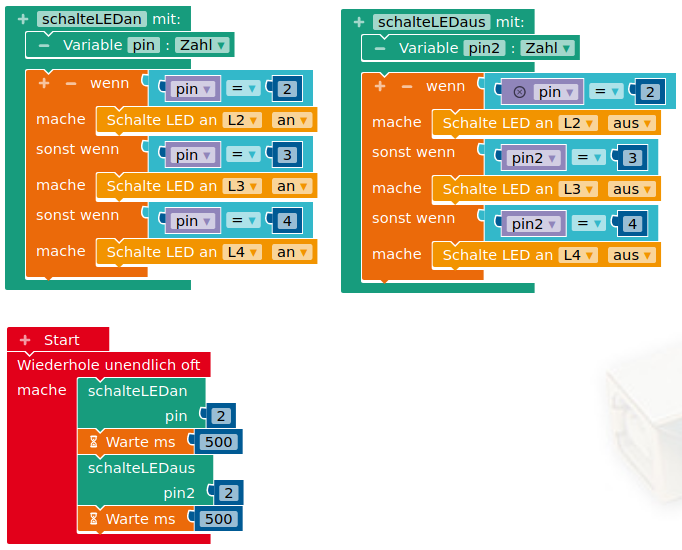
\includegraphics[width=\linewidth]{./pics/eigene-funktion-demo.png}
\end{figure}

\newpage
% Funktion blinke x mal mit pause p
\begin{aufgabe} \emph{Block zum Blinken}
	
	Implementiere einen Block \texttt{blinke} mit den Argumenten \texttt{anzahl} und \texttt{pauseInMSek}, die die Board-LED für die angegebene Anzahl und mit der angegebenen Pause in Millisekunden zum Blinken bringt. Überprüfe deinen Block.
	
	Was passiert, wenn eine Kommazahl übergeben wird?
\end{aufgabe}

\begin{aufgabe} \emph{Lesbarkeit und Rückgabewerte}
	
	Die Logik für die Straßenlaterne (vgl. S. \pageref{proj:strassenlampe}) lautete: Wenn es dunkel ist, schalte die Lampe an, sonst schalte die Lampe aus.
	
	\begin{wrapfigure}{r}{0.3\linewidth}
		\centering
		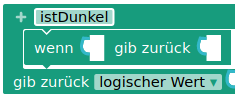
\includegraphics[width=\linewidth]{./pics/istDunkel.png}
	\end{wrapfigure}
	Mit einem eigenen Block lässt sich diese Logik direkt im Programm umsetzen, sodass es noch besser lesbar wird. Implementiere einen Block \texttt{istDunkel}, der basierend auf den Werten eines angeschlossenen LDR an A0 einen Wahrheitswert zurückgibt.
	
	\emph{Tipp:} Nutze ggf. die \nepohilfe Hilfefunktion auf der rechten Seite, um dich mit den abgebildeten Blöcken vertraut zu machen.
\end{aufgabe}

\bigskip
\begin{zsfg}{Funktionen}
	
	\begin{wrapfigure}{r}{0.65\textwidth}
		\centering
		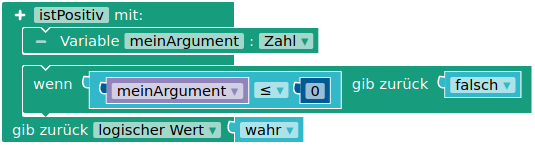
\includegraphics[width=\linewidth]{./pics/istPositiv.png}
	\end{wrapfigure}
	Funktionen fassen mehrere Anweisungen zusammen und können als eigene Anweisung im Algorithmus genutzt werden, um ihn lesbarer und modularer zu machen, wenn an einigen Stellen die gleichen Anweisungen immer wieder benötigt werden. Für den Namen der Funktion gilt wiederum die \href{https://de.wikipedia.org/wiki/Binnenmajuskel#Programmiersprachen}{lowerCamelCase}-Konvention.
	
	Funktionen können mehrere Argumente von unterschiedlichem Typ haben, die die Art der Ausführung variieren können. Die Variablen, in denen diese Argumente gespeichert werden, sind lokale Variablen und daher nur innerhalb der Funktion verfügbar.
	
	Außerdem können Funktionen einen Wert zurückgeben, der für den \enquote{Hauptalgorithmus} genutzt werden kann. Die Rückgabe eines Wertes muss nicht am Ende der Funktion erfolgen. Wenn bereits vor dem Ende ein Wert zurückgegeben wird, wird der Rest der Funktion nicht mehr ausgeführt.
\end{zsfg}

% Funktionen mit Rückgabewerten: Berechnung einer Zahl, Überprüfung einer Gültigkeit
Die Bezeichnung \enquote{Computer}, zu deutsch: \enquote{Rechner}, besagt schon, dass man die Entwicklung von Mikrocontrollern und Mikroprozessoren immer auch dazu diente, Rechnungen zu automatisieren, die ein Rechner wesentlich schneller, präziser und fehlerfreier vornehmen kann als ein Mensch. Die Grundrechenarten sind schon als Blöcke in Nepo implementiert. Damit lassen sich auch auf schnelle Art weitere Berechnungen anstellen, für die ein Mensch mehrere Minuten oder sogar Stunden bräuchte.

\begin{aufgabe} \emph{Teilbarkeit durch 2}
	
	Unten ist ein Programm abgebildet, mit dem die Teilbarkeit durch 2 überprüft wird. Erläutere seinen Ablauf.
\end{aufgabe}

\begin{figure}[H]
	\centering
	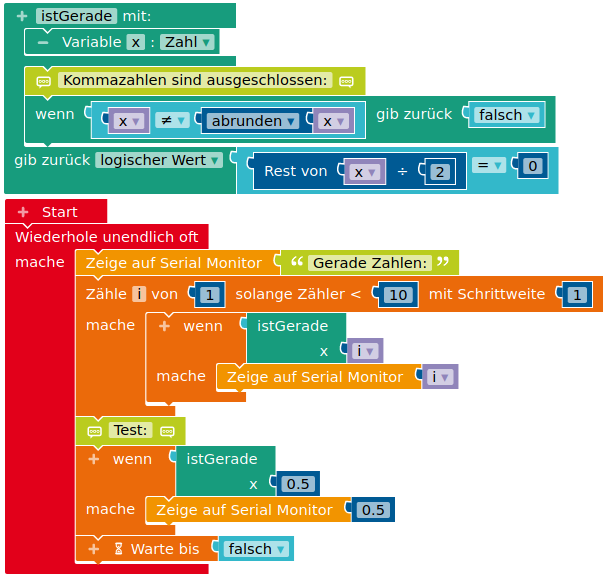
\includegraphics[width=0.7\linewidth]{./pics/istGerade.png}
\end{figure}

% Gültigkeit: Funktion istPrimzahl(Zahl)  (naiver Test)
\begin{aufgabe} \emph{Primzahlen}
	
	Primzahlen sind natürliche Zahlen, die nur durch 1 und sich selbst teilbar sind. Die kleinste mögliche Primzahl ist 2.
	
	Primzahlen haben die Menschen seit jeher fasziniert, weil man bis heute keine Formel gefunden hat, um Primzahlen zu berechnen. Im Wesentlichen ist man darauf angewiesen, alle möglichen Teiler auszuprobieren und auf diese Art herauszufinden, ob eine Zahl eine Primzahl ist oder nicht. Unter anderem aufgrund dieser \enquote{Sperrigkeit} eignen sich Primzahlen gut zur Verschlüsselung.
	
	\medskip
	\begin{wrapfigure}{r}{0.2\linewidth}
		\centering
		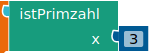
\includegraphics[width=\linewidth]{./pics/istPrimzahl-Block.png}
	\end{wrapfigure}
	Implementiere einen Block \texttt{istPrimzahl} mit einer Zahl \texttt{x} als Argument und einem Wahrheitswert als Rückgabewert. Sorge dafür, dass Kommazahlen sofort als falsch erkannt werden. Für den Primzahltest kannst du zunächst für alle Zahlen von 2 bis $x-1$ überprüfen, ob sie Teiler von $x$ sind. Der Mathe-Block \texttt{\dots ist Primzahl} darf nicht verwendet werden - es geht hier darum, ihn selbst zu implementieren.
	
	Implementiere dann ein Programm, das alle Primzahlen zwischen 1 und 1000 ausgibt. Füge einen Primzahlzähler ein, der am Ende ausgibt, wie viele Primzahlen gefunden wurden. Recherchiere, ob dein Programm das korrekte Ergebnis liefert.
	%korrekt: 168
	
	\bigskip
	\emph{Zusatz:} Bei größeren Zahlen braucht der Arduino schon relativ lange, um alle Rechenschritte durchzuführen. Dies führt zu einem typischen Problem der Informatik:
	\begin{center}
		\emph{Wie kann man ein Verfahren so optimieren, dass es auch bei begrenzter Rechenkapazität annehmbar schnell abgearbeitet wird?}
	\end{center}
	
	Überlege dir Antworten zu folgenden Fragen und optimiere dein Programm entsprechend:
	\begin{enumerate}[label=\alph*), itemsep=0ex, parsep=0ex]
		\item Wie groß kann ein Teiler von x maximal sein?
		\item Zu einem Teiler $t_1$ gehört immer ein zweiter Teiler $t_2$ mit $t_1 \cdot t_2 = x$. Zum Beispiel ist $9$ ein Teiler von $18$ und ein zweiter zugehöriger Teiler ist $2$, denn $2\cdot 9 = 18$. Die Überprüfung der Teiler von 18 muss aber nicht bis 9 gehen, weil die Überprüfung der 2 in diesem Fall schon ausreicht. Wie groß ist der größte Teiler, der nicht schon durch einen zugehörigen kleineren Teiler gefunden werden kann? Denke zum Beispiel an die Teiler von 36.
	\end{enumerate}
\end{aufgabe}

% Fibonacci Zahlen der Reihe nach ausgeben
% n-te Fibonacci Zahl berechnen und zurückgeben
% dabei mit Argument steuern, ob es eine Ausgabe aller Zwischenberechnungen geben soll oder nicht

\begin{aufgabe} \emph{Berechnungen zur Fibonacci-Folge}
	
	\begin{wrapfigure}{r}{0.3\textwidth}
		\vspace{-0.5\baselineskip}
		\centering
		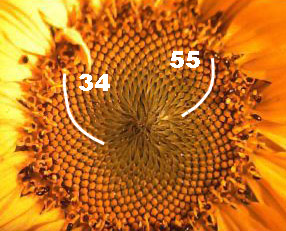
\includegraphics[width=0.3\textwidth]{./pics/fibonacci-sonnenblume.jpg}
		\caption{Fibonacci-Zahlen finden sich in den Blütenständen von vielen Blumen. (\href{https://de.wikipedia.org/wiki/Datei:Goldener_Schnitt_Bluetenstand_Sonnenblume.jpg}{Bild: CC-BY-SA, Urheber Dr. Helmut Haß})}
		\vspace{-4\baselineskip}
	\end{wrapfigure}
	Die \href{https://de.wikipedia.org/wiki/Fibonacci-Folge}{Fibonacci-Folge} beginnt mit den Zahlen $f_1 = 1$ und $f_2 = 1$. Die darauf folgende Zahl ist die Summe der beiden vorhergehenden Zahlen:
	\begin{align*}
		f_3 &= f_1 + f_2 = 2 \\
		f_4 &= f_2 + f_3 = 3 \\
		&\dots \\
		f_n &= f_{n-1} + f_{n-2}
	\end{align*}
	
	\begin{enumerate}[label=\alph*), itemsep=0ex, parsep=0ex]
		\item Berechne schriftlich die ersten 10 Glieder der Fibonacci-Folge.
		\item Implementiere einen Block \texttt{gibFibonaccizahl} mit einem Argument \texttt{n}, das angibt, die wie vielte Fibonacci-Zahl berechnet werden soll, und einem Argument \texttt{mitAusgabe}, das angibt, ob eine Ausgabe der vorhergehenden Folgenglieder bei der Berechnung erfolgen soll oder nicht. Die n-te Fibonacci-Zahl wird zurückgegeben.
	\end{enumerate}
\end{aufgabe}

\newpage
\section{Debugging: Fehler im Programm finden}
\label{sec:debugging}

Fehler werden in der Informatik auch als \enquote{Bugs} bezeichnet. Fehler treten beim Programmieren ständig auf und sind völlig normal. Erst nach einigem Testen läuft ein Programm völlig stabil und fehlerfrei. Das Entfernen von Fehlern wird dann auch als \enquote{Debugging} bezeichnet. 

Informatiker unterscheiden zwischen zwei Fehlerarten: Syntaxfehler und logische Fehler. Logische Fehler sind dir vielleicht schon passiert und manche wurden auch schon in diesem Skript behandelt, zum Beispiel zur \texttt{sonst wenn}-Bedingung auf S.\,\pageref{abb:sonstWenn1}. Syntaxfehler entstehen, wenn man die Grammatik (Syntax) einer Programmiersprache nicht beachtet. In Nepo werden die meisten Syntaxfehler automatisch vermieden, weil die meisten Blöcke nur ineinander greifen, wenn sie syntaktisch zueinander passen.

Unten ist ein Programm mit zwei Fehlern abgebildet. Es soll die folgende Summe berechnen:
\begin{equation*}
	1 + 1,5 + 2 + 2,5 + 3 + \dots + 98,5 + 99 + 99,5 + 100.
\end{equation*}

\begin{figure}[H]
	\centering
	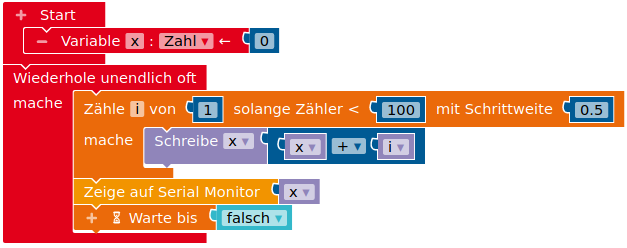
\includegraphics[width=0.7\linewidth]{./pics/debugBsp.png}
	\caption{Beispielprogramm zum Debuggen: \textattachfile[mimetype=text/plain, description={Vorlage zum Debuggen}]{./lsg/NEPO-Debug-Bsp.xml}{
			Debug-Bsp.xml%
	}}
\end{figure}

\begin{aufgabe}
	
	\begin{wrapfigure}{r}{0.4\textwidth}
		\centering
		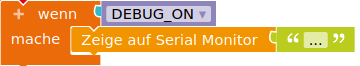
\includegraphics[width=\linewidth]{./pics/DEBUGON.png}
	\end{wrapfigure}
	Um Fehler zu finden, kann man sich die Werte von Variablen auf dem seriellen Monitor ausgeben lassen. Programmierer bauen dann häufig eine Variable \texttt{DEBUG\_ON} ein und nutzen eine Konstruktion wie rechts abgebildet. Welchen Vorteil könnte das haben?
	
	Öffne das oben abgebildete Programm in Nepo und nutze die Debug-Konstruktion, um die Fehler zu finden oder nachzuweisen. Korrigiere sie.
	
	\emph{Frage deinen Lehrer, wenn du den Fehler gefunden hast, aber nicht nachvollziehen kannst, wieso sich das Programm so verhält.}
\end{aufgabe}

\newpage
\section{Das EVA-Prinzip}
\label{sec:eva}

In diesem Kapitel hast du bereits einige Bauteile kennengelernt, aber es gibt noch viele mehr. Um dabei nicht den Überblick zu verlieren, wären Kategorien praktisch, mit denen man Bauteile und informationsverarbeitende Systeme im Allgemeinen einordnen kann.

\begin{ziel}
	\textbf{Frage:} Wie lassen sich elektrische Bauteile und informationsverarbeitende Systeme kategorisieren?
\end{ziel}

\marginpar{%
	\textattachfile[description={Folie zu Kap. \thechapter, informationsverarbeitende Systeme}]{./Auftraege/kap3-auftrag-infoverarbeitung.pdf}{%
		\footnotesize\folie Folie%
	}%
	\footnotesize%
	\\öffnen%
}
\begin{aufgabe} \emph{Informationsverarbeitung}
	
	Lies die beiden Beschreibungen zur Informationsverarbeitung bei der Straßenlampe und beim Menschen. Beschreibe Gemeinsamkeiten.
\end{aufgabe}

\bigskip

\begin{tabu} to \textwidth {X[L]X[L]}
	\emph{\bfseries Beispiel Dämmerungsschaltung:}
	
	Der Aufbau von Festwiderstand und LDR ermöglicht die Eingabe von Daten zur Helligkeit. Auf dem Arduino werden die elektrischen Signale entsprechend des laufenden Programms verarbeitet. Letztlich erfolgt die Ausgabe durch das Leuchten einer LED, wenn es dunkel ist, bzw. durch das Nicht-Leuchten der LED.
	
	&
	
	\emph{\bfseries Beispiel Mensch:}
	
	Unsere Sinne (Augen zum Sehen, Ohren zum Hören, \dots) ermöglichen die Eingabe von Informationen in das System Mensch. Im Gehirn und den weiteren Nervenbahnen im Körper werden die Signale verarbeitet. Schließlich kommt es zu einer Ausgabe - zum Beispiel zu einer Bewegung (Musik leiser drehen, Augen zukneifen, sprechen mit dem Mund \dots).
	\\
\end{tabu}

\bigskip

\begin{zsfg}{Das EVA-Prinzip}
	
	Informationsverarbeitende Systeme lassen sich nach ihrer Funktion in drei Einheiten zerlegen: Eingabeeinheit, Verarbeitungseinheit, Ausgabeeinheit.
	
	\bigskip
	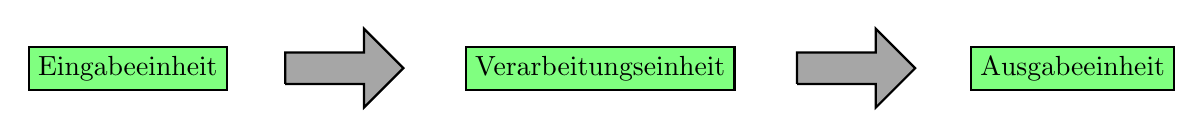
\begin{tikzpicture}[rect/.style={shape=rectangle, thick, draw=black, fill=green!50}]
	\node at (0,0) [rect] {Eingabeeinheit};
	\draw [fill=gray!70, thick] (2,-0.2) -- ++(1,0)-- ++(0,-0.3) -- ++(0.5,0.5) -- ++(-0.5,0.5) -- ++(0,-0.3) -- ++(-1,0) -- ++(0,-0.4);
	\node at (6,0) [rect] {Verarbeitungseinheit};
	\draw [fill=gray!70, thick] (8.5,-0.2) -- ++(1,0)-- ++(0,-0.3) -- ++(0.5,0.5) -- ++(-0.5,0.5) -- ++(0,-0.3) -- ++(-1,0) -- ++(0,-0.4);
	\node at (12,0) [rect] {Ausgabeeinheit};
	\end{tikzpicture}
	
	\bigskip
	Mit dem EVA-Prinzip wird die grundlegende Reihenfolge der Verarbeitung von Daten charakterisiert. Die Einheiten bestehen dabei nicht nur aus den Bauteilen, sondern beinhalten auch die Art der Verarbeitung, also zum Beispiel das Programm auf dem Arduino. 
\end{zsfg}

\begin{aufgabe} \emph{Kleines Begriffstraining}
	
	\begin{enumerate}[label=\alph*),itemsep=0ex,parsep=0ex]
		\item Kategorisiere die \emph{Juke-Box} (s. S. \pageref{proj:jukebox}) nach dem EVA-Prinzip.
		\item Kategorisiere den \emph{Reaktionszeitmesser} (s. S. \pageref{proj:reaktionszeitmesser}) nach dem EVA-Prinzip.
	\end{enumerate}
\end{aufgabe}

\newpage

\marginpar{%
	\textattachfile[description={Folie zu Kap. \thechapter, Bauteilkategorisierung}]{./Auftraege/kap3-bauteilkategorisierung.pdf}{%
		\footnotesize\folie Folie%
	}%
	\footnotesize%
	\\öffnen%
}
\begin{aufgabe}
	Du hast bisher (mindestens) folgende Bauteile verwendet:
	
	\medskip
	\begin{center}
		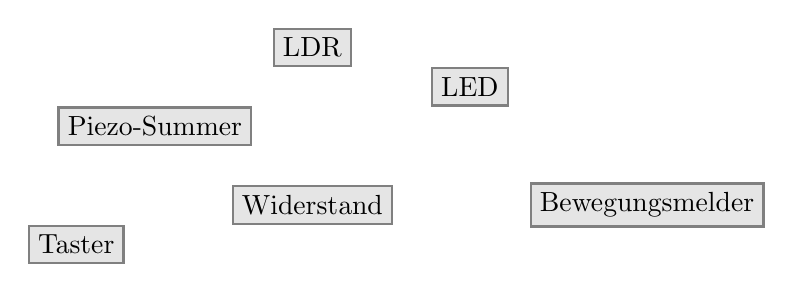
\begin{tikzpicture}[rect/.style={shape=rectangle, thick, draw=black!50, fill=black!10}]
		\node at (5,2) [rect] {LED};
		\node at (3,0.5) [rect] {Widerstand};
		\node at (0,0) [rect] {Taster};	
		\node at (1,1.5) [rect] {Piezo-Summer};
		\node at (3,2.5) [rect] {LDR};
		\node at (7.25,0.5) [rect] {Bewegungsmelder};
		\end{tikzpicture}
	\end{center}
	
	\medskip
	Benenne Gemeinsamkeiten und Unterschiede. Welche Bauteile lassen sich zusammenfassen?
\end{aufgabe}

\bigskip
\begin{zsfg}{Sensoren und Aktoren mit digitalen und analogen Signalen}
	Für die Eingabe von Daten werden \emph{Sensoren} benötigt; für die Ausgabe hingegen \emph{Aktoren}:
	\begin{itemize}[itemsep=0mm,parsep=0mm]
		\item \textbf{Sensoren} (auch Fühler genannt) sind elektrische Bauteile, die eine physikalische Größe aus der Umwelt (Temperatur, Helligkeit, Luftdruck oder auch ein mechanischer Druck mit dem Finger) in eine elektrische Größe (Widerstand, Spannung, elektrisches Potential, Stromstärke) umwandeln. Dadurch werden die physikalischen Größen aus der Umwelt einer elektronischen Verarbeitung zugänglich.
		\item \textbf{Aktoren} (auch Aktuatoren genannt) sind elektrische Bauteile, die eine elektrische Größe in eine mechanische (Bewegung, Schallwellen) oder andere Größe (Temperatur, Licht, \dots) umwandeln. Sie ermöglichen, dass die elektronische Verarbeitung zu Handlungen bzw. Konsequenzen führen kann.
	\end{itemize} 
	
	\medskip
	Die Signale von Sensoren und Aktoren können digital oder analog sein:
	\begin{itemize}[itemsep=0ex, parsep=0ex]
		\item \textbf{Digitale Signale} haben nur zwei mögliche Zustände - z.\,B. an / aus, gedrückt / nicht gedrückt oder 1 / 0.
		\item \textbf{Analoge Signale} haben unendlich viele mögliche Werte, weil sie beliebig fein eingeteilt werden können. Digitale Geräte wie der Arduino können nur \emph{quasi} analoge Signale einlesen. Bei den \enquote{analogen} Eingängen A0, A1, \dots A5 des Arduino sind 1024 verschiedene Stufen möglich; bei \enquote{analogen} Ausgängen (Pins mit einer Tilde: $\sim$) sind 256 verschiedene Stufen möglich. Diese Einteilung ist für die meisten Aufgaben fein genug.
	\end{itemize}
	
	\begin{figure}[H]
		\centering
		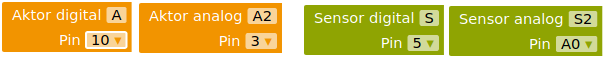
\includegraphics[width=0.8\linewidth]{./pics/sensoren-und-aktoren.png}
		\caption{Digitale und analoge Aktoren und Sensoren in Nepo.}
	\end{figure}
\end{zsfg}

\bigskip

\begin{projekt}[Alarmanlage mit Lichtschranke]\label{proj:alarmanlage}
	\begin{minipage}{0.78\textwidth}
		Baue eine Alarmanlage, indem du mit einer LED (Vorwiderstand!) und einem LDR eine Lichtschranke baust . Wird diese unterbrochen, soll ein akustischer Alarm ertönen. Über einen zusätzlichen Taster (mit Widerstand!) soll die Alarmanlage \enquote{scharf} gestellt bzw. wieder ausgestellt werden können.
	\end{minipage}
	\hfill
	\begin{minipage}{0.2\textwidth}
		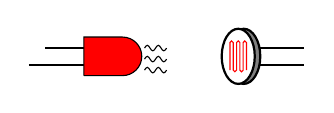
\begin{tikzpicture}[scale=0.7]
		%LED
		\draw [thick] (0,0) -- (1,0);
		\draw [thick] (0.3,0.3) -- (1,0.3);
		\draw [fill=red] (1,-0.2) -- (1,0.5) -- (1.7,0.5) arc [start angle=90,end angle=-90,radius=0.35] -- (1,-0.2);
		%Lichtstrahlen
		\draw (2.1,-0.1) sin ++(0.05,0.05) cos ++(0.05,-0.05) sin ++(0.05,-0.05) cos ++(0.05,0.05) sin ++(0.05,0.05) cos ++(0.05,-0.05) sin ++(0.05,-0.05) cos ++(0.05,0.05);
		\draw (2.1,0.1) sin ++(0.05,0.05) cos ++(0.05,-0.05) sin ++(0.05,-0.05) cos ++(0.05,0.05) sin ++(0.05,0.05) cos ++(0.05,-0.05) sin ++(0.05,-0.05) cos ++(0.05,0.05);
		\draw (2.1,0.3) sin ++(0.05,0.05) cos ++(0.05,-0.05) sin ++(0.05,-0.05) cos ++(0.05,0.05) sin ++(0.05,0.05) cos ++(0.05,-0.05) sin ++(0.05,-0.05) cos ++(0.05,0.05);
		% LDR
		\draw [thick] (4,0) -- (5,0);
		\draw [thick] (4,0.3) -- (5,0.3);
		\draw [thick,fill=gray] (3.9,0.15) ellipse [x radius=0.3,y radius=0.5];
		\draw [thick,fill=white] (3.8,0.15) ellipse [x radius=0.3,y radius=0.5];
		\draw [red] (3.65,-0.1) -- ++(0,0.5) arc [start angle=-180,end angle=-360,radius=0.03] -- ++(0,-0.5) arc [start angle=-180,end angle=0,radius=0.03] -- ++(0,0.5) arc [start angle=-180,end angle=-360,radius=0.03] -- ++(0,-0.5) arc [start angle=-180,end angle=0,radius=0.03] -- ++(0,0.5) arc [start angle=-180,end angle=-360,radius=0.03] -- ++(0,-0.5);
		\end{tikzpicture}
	\end{minipage}
\end{projekt}


\begin{minipage}{0.6\textwidth}
	\emph{Hinweise:}
	
	Konfiguriere alle benötigten Bauteile als Aktoren und Sensoren.
	
	\medskip
	\footnotesize%
	Links: \quad \zurueck \hyperref[abb:schaltplan-taster]{Taster anschließen}, \quad \zurueck \hyperref[abb:schaltplan-ldr]{LDR anschließen}
\end{minipage}
\hfill
\begin{minipage}{0.38\textwidth}
	\begin{figure}[H]
		\centering
		
\includegraphics[width=0.9\linewidth]{./pics/aktor-ansteuern.png}
		\includegraphics[width=0.9\linewidth]{./pics/sensor-auslesen.png}
		%\caption{Blöcke zum Ansteuern und Auslesen von Aktoren und Sensoren.}
	\end{figure}
\end{minipage}

\vspace{3\baselineskip}
\begin{aufgabe} \emph{Analoge Aktoren}
	
	Analoge Aktoren kamen bisher nicht vor. Schließe eine LED mit Vorwiderstand an Pin 5 an und konfiguriere einen entsprechenden analogen Aktor.
	
	\begin{enumerate}[label=\alph*), itemsep=0ex, parsep=0ex]
		\item An Pin 5 können Werte von 0 bis 255 ausgegeben werden. Implementiere eine Zählschleife, die diese Werte systematisch durchläuft und beschreibe die Auswirkung auf die LED.
		\item Probiere Werte größer als 255 aus und beschreibe, welche Auswirkung diese haben.
	\end{enumerate}
\end{aufgabe}


\newpage
\section{Vermischte Übungen}
\label{sec:algo-uebungen}

% TODO: vermischte Übungen ergänzen
% Komplexere Juke-Box
% 

% Vier Taster angeschlossen; Kombinationen von logischen Operationen durchdenken lassen
% Form:
% Wenn x und y oder z oder nicht a
% 	Serial Monitor: Du bist drin
% Sonst
% 	Serial Monitor: Leider falsch

% Gesetze von de Morgan

% Collatz-Zahl


\newpage
\section{Ausblick}
\label{sec:algo-ausblick}

\begin{ziel}
	\textbf{Offene Fragen:}
	
	\begin{itemize}[itemsep=0ex,parsep=0ex]
		\item Was passiert, wenn ein Digitalpin angestellt oder ausgestellt wird?
		
		$\rightarrow$ \hyperref[kap:elektrischegrundlagen]{Kap.: Elektrische Grundlagen}
		\item Was passiert bei der Messung der Lichtstärke?
		
		$\rightarrow$ \hyperref[kap:elektrischegrundlagen]{Kap.: Elektrische Grundlagen}
		\item Wie werden weitere Bauteile angeschlossen und im Programm angesprochen?
		
		$\rightarrow$ \hyperref[kap:bauteilkunde]{Kap.: Bauteilkunde}
		\item Was sind Listen und wie verwendet man sie?
		\item Wie werden die Daten codiert, um sie auf dem Arduino abzuspeichern oder zwischen Arduino und Computer auszutauschen?
	\end{itemize}
\end{ziel}

%TODO: Verweis von den Fragen zu kommenden Kapiteln

%Weitere Fragen für später:
%
% Wie lässt sich der Arduino textbasiert programmieren? -> Textbasiertes Programmieren (am Ende von Kap. zu Codierung?)
% Wie lassen sich komplexere Maschinen programmieren? -> Automaten, Steuern und Regeln (am Ende von Kap. Werkzeugkasten)


\vfill
\begin{links}
	\item \href{https://www.heise.de/make/meldung/Schueler-Projekt-Selbstbau-Staubsaugerroboter-aus-dem-3D-Drucker-3991208.html}{Staubsaugerroboter}
	
	Mithilfe eines Arduino haben zwei Schüler aus den Niederlanden ihren eigenen Staubsaugerroboter gebaut. Das Teile für das Gehäuse haben sie mit einem 3D-Drucker gedruckt.
	
	\item \href{https://www.heise.de/make/artikel/Einfacher-Ultraschall-Levitationsapparat-4022505.html}{Levitation}
	
	Durch Levitation lassen sich Gegenstände scheinbar von Geisterhand in der Luft schweben. Die nötige Elektronik dafür lässt sich mit einem Arduino realisieren.
	
	\item \href{https://www.instructables.com/id/Party-Lights-1/}{Arduino-kontrollierter LED-Streifen zur Visualisierung von Musik}
	
	Der Arduino lässt sich zudem über ein Smartphone ansteuern.
	
	\item \href{https://www.heise.de/make/meldung/Makerbuino-Spielkonsole-fuer-den-Eigenbau-3681578.html}{Spielekonsole von Makerbuino}
	
	Mithilfe eines Bausatzes lässt sich eine kleine, Arduino-basierte Spielekonsole bauen.
\end{links}